\documentclass[conference]{IEEEtran}
\IEEEoverridecommandlockouts

\usepackage{cite}
\usepackage{amsmath,amssymb}
\usepackage{graphicx}
\usepackage{booktabs}
\usepackage{multirow}
\usepackage[table]{xcolor}
\usepackage{tikz}
\usetikzlibrary{arrows.meta,positioning,fit,backgrounds,calc}
\usepackage{pgfplots}
\pgfplotsset{compat=1.18}
\usepackage{algorithm}
\usepackage{algpseudocode}
\usepackage{url}

% ---- things the team still has to fill in show up in red ----
\newcommand{\fillme}[1]{\textcolor{red}{[#1]}}

% ---- level tile colours (Fig. 4) ----
\definecolor{lfwall}{HTML}{3A3F4B}
\definecolor{lfstart}{HTML}{2E9E4F}
\definecolor{lfexit}{HTML}{2B6CD8}
\definecolor{lfkey}{HTML}{C03BC8}
\definecolor{lfdoor}{HTML}{8A5A2B}
\definecolor{lfmon}{HTML}{D7263D}
\definecolor{lftrap}{HTML}{F08A24}
\definecolor{lfpot}{HTML}{3CC8B4}
\definecolor{lfcoin}{HTML}{E8C21B}
% ---- architecture colours (Fig. 1) ----
\definecolor{cgen}{HTML}{EDE4FB}
\definecolor{cagent}{HTML}{E2EEFB}
\definecolor{cmca}{HTML}{FDEBD8}
\definecolor{cio}{HTML}{F1F1F1}

\begin{document}

\title{LevelForge: An Agentic Digital Twin Framework for Feedback-Driven Autonomous Game-Level Generation and Optimization}

\author{
\IEEEauthorblockN{Swastik Dasgupta, \fillme{Team member 2}, \fillme{Team member 3}, \fillme{Team member 4}}
\IEEEauthorblockA{Department of Artificial Intelligence and Machine Learning\\
M S Ramaiah Institute of Technology, Bengaluru, India\\
\fillme{email addresses}}
}

\maketitle

\begin{abstract}
Players often complain that a particular game level is too hard, confusing or unfair, but turning
those complaints into a better level is slow, manual work that needs many rounds of play-testing.
We present LevelForge, a framework that takes a problem level and its player reviews, places the
level in a sandboxed \emph{digital twin}, and lets AI agents redesign it. A large language model
(LLM) first mines the reviews into a taxonomy of design problems and derives measurable design
targets. \emph{Design agents} (generator, critic and optimiser, orchestrated as a LangGraph state
machine) then propose alternative structured edits, and every candidate level is play-tested by
hundreds of \emph{player agents} with three distinct play styles. Because each simulated
playthrough is independent, play-testing runs simultaneously on a multicore process pool, evaluating
up to 11,250 playthroughs per optimisation run in seconds. The developer receives the optimised
level, the reasons behind each accepted change, and per-player-type statistics. On 12 starting
levels with an identical simulation budget, critic-guided optimisation raised mean quality from
0.572 to 0.783 (+37\%) and beat random search on 9 of 12 levels (Wilcoxon $p=0.034$), matching
random search's final quality with two thirds of the budget. Parallel play-testing reached a
$3.71\times$ speedup on 5 workers and $6.47\times$ on 12 logical cores, with an experimentally
determined serial fraction of 0.086. LLM-driven design agents performed comparably to hand-written
rules while also designing levels from scratch and explaining their changes in natural language.
\end{abstract}

\begin{IEEEkeywords}
procedural content generation, agentic AI, large language models, digital twin, automated play-testing, multicore parallelism
\end{IEEEkeywords}

% =====================================================================
\section{Introduction}
% =====================================================================
Game developers receive a constant stream of player feedback. On Steam alone, reviews are numerous,
and negative reviews in particular contain specific, actionable complaints~\cite{lin2019steam}:
``the second floor is way too hard'', ``I kept getting lost'', ``traps on the only path are unfair''.
Fixing a level in response is still largely manual. A designer has to interpret the complaints,
guess which change would address them, edit the level, and play-test it again, often many times,
because a change that fixes one complaint can cause another.

This paper asks whether that loop can be automated. Our approach follows the workflow a designer
would use, but replaces each manual step with an AI component:
\begin{enumerate}
\item \textbf{Listen:} an LLM reads the player reviews of a problem level and turns them into
measurable design targets (\emph{Generative AI}).
\item \textbf{Sandbox:} the level is loaded into a digital twin~\cite{grieves2017twin} of the
game, a fast, simplified simulation that keeps the level layout and game values.
\item \textbf{Redesign:} design agents diagnose the level's weaknesses and propose several
alternative edits per round (\emph{agentic AI}).
\item \textbf{Play-test:} hundreds of player agents play every candidate level simultaneously on
all CPU cores (\emph{multicore architecture}).
\item \textbf{Report:} the developer receives the optimised level together with an explanation
of what changed and why, so the fix can be reviewed and learned from rather than applied blindly.
\end{enumerate}

LLMs can already generate game levels~\cite{todd2023level,sudhakaran2023mariogpt}, but generation
alone does not guarantee that a level is playable, balanced or aligned with what players asked for.
Judging that needs many playthroughs, which is computationally expensive. LevelForge therefore
combines LLM reasoning with large-scale parallel simulation, and keeps the LLM in a reasoning role
while a deterministic validator guarantees that every level stays playable.

\textbf{Contributions.}
(i)~A review-to-brief pipeline that converts free-text player feedback into quantitative design
targets and objective weights.
(ii)~A two-tier multi-agent system: LLM \emph{design agents} in a generate--simulate--critique--optimise
loop with structured, validated edits, simulation feedback and a reflection memory; and rule-based
\emph{player agents} that play-test in the digital twin.
(iii)~A parallel Monte-Carlo play-testing engine on a multicore process pool, with a scaling and
task-granularity study.
(iv)~A controlled comparison of rule-based reasoning, LLM reasoning and random search under the
same simulation budget and starting levels.
(v)~A developer-facing output: a report, natural-language designer notes, and a playable
first-person 3D game built from the generated levels.

% =====================================================================
\section{Related Work}
% =====================================================================
\textbf{Procedural content generation (PCG).} Search-based PCG optimises content against an
evaluation function, often with evolutionary search~\cite{togelius2011sbpcg,shaker2016pcg}.
Experience-driven PCG models the player's experience and generates content to shape
it~\cite{yannakakis2011edpcg}. We follow the search-based framing, but derive the evaluation
function from player reviews, and use an agent loop with diagnosis instead of blind variation.

\textbf{Machine learning and LLMs for levels.} PCG via machine learning learns content from
existing examples~\cite{summerville2018pcgml}. Fine-tuned language models generate Sokoban
levels~\cite{todd2023level} and Super Mario levels from text prompts~\cite{sudhakaran2023mariogpt}.
These works focus on generating new levels; we focus on \emph{repairing} an existing problem level
in response to feedback, with simulation in the loop.

\textbf{Automated play-testing.} Procedural personas use agents with different objectives to
represent different play styles~\cite{holmgard2019personas}. Our player agents follow this idea
with three cost-based planning personas, and use the gap between them as a measure of skill
expression.

\textbf{LLM agents and annotation.} ReAct interleaves reasoning and actions~\cite{yao2023react}, and
Reflexion keeps a verbal memory of failed attempts~\cite{shinn2023reflexion}; our critic's memory of
failed fixes is a lightweight form of the latter. LLMs have been shown to match or outperform crowd
workers on text annotation~\cite{gilardi2023annotation}, which motivates LLM-based review labelling.

\textbf{Parallel performance.} We analyse scaling with Amdahl's law~\cite{amdahl1967} and the
Karp--Flatt experimentally determined serial fraction~\cite{karpflatt1990}.

% =====================================================================
\section{System Overview}
% =====================================================================
Fig.~\ref{fig:arch} shows the pipeline. Its input is a level and the player reviews of that level;
alternatively, the generator agent can design a first level from the reviews alone. Two kinds of
agents work together (Table~\ref{tab:agents}): design agents decide \emph{what to change}, and
player agents measure \emph{whether the change worked}.

\begin{figure*}[t]
\centering
\resizebox{\textwidth}{!}{%
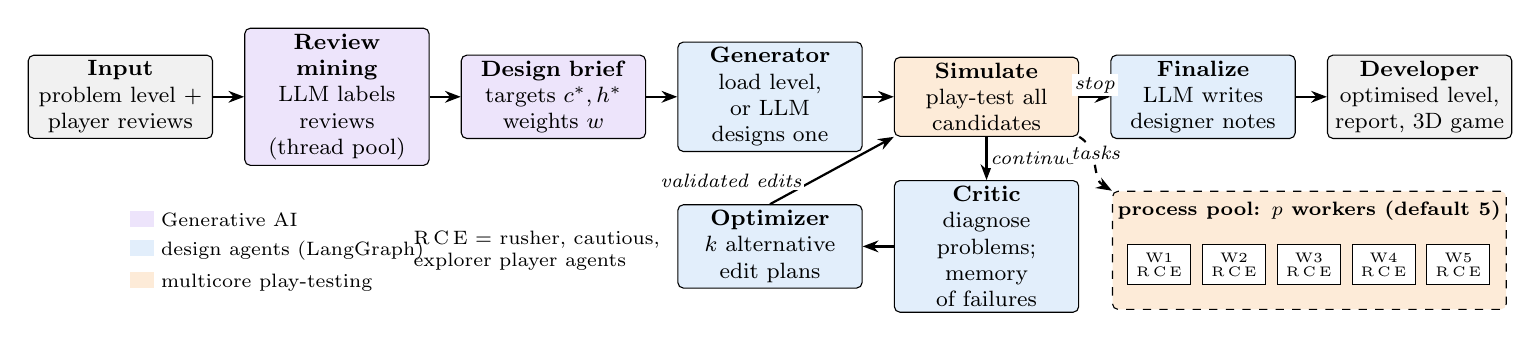
\begin{tikzpicture}[
  font=\footnotesize,
  box/.style={draw, rounded corners=2pt, align=center, minimum height=10mm, text width=22mm, inner sep=2pt},
  arr/.style={-{Stealth[length=2mm]}, thick},
  lab/.style={font=\scriptsize\itshape, fill=white, inner sep=1pt}
]
\node[box, fill=cio]    (in)   at (0,0)    {\textbf{Input}\\problem level +\\player reviews};
\node[box, fill=cgen]   (mine) at (2.75,0) {\textbf{Review mining}\\LLM labels reviews\\(thread pool)};
\node[box, fill=cgen]   (brief)at (5.5,0)  {\textbf{Design brief}\\targets $c^*, h^*$\\weights $w$};
\node[box, fill=cagent] (gen)  at (8.25,0) {\textbf{Generator}\\load level, or LLM\\designs one};
\node[box, fill=cmca]   (sim)  at (11,0)   {\textbf{Simulate}\\play-test all\\candidates};
\node[box, fill=cagent] (fin)  at (13.75,0){\textbf{Finalize}\\LLM writes\\designer notes};
\node[box, fill=cio]    (out)  at (16.5,0) {\textbf{Developer}\\optimised level,\\report, 3D game};
\node[box, fill=cagent] (crit) at (11,-1.9) {\textbf{Critic}\\diagnose problems;\\memory of failures};
\node[box, fill=cagent] (opt)  at (8.25,-1.9){\textbf{Optimizer}\\$k$ alternative\\edit plans};

\draw[arr] (in) -- (mine);
\draw[arr] (mine) -- (brief);
\draw[arr] (brief) -- (gen);
\draw[arr] (gen) -- (sim);
\draw[arr] (sim) -- node[lab, above]{stop} (fin);
\draw[arr] (fin) -- (out);
\draw[arr] (sim) -- node[lab, right]{continue} (crit);
\draw[arr] (crit) -- (opt);
\draw[arr] (opt.north) -- node[lab, pos=0.35, left=1mm]{validated edits} (sim.south west);

% process pool
\node[draw, dashed, rounded corners=2pt, fill=cmca, minimum width=50mm, minimum height=15mm] (pool) at (15.1,-1.95) {};
\node[font=\scriptsize\bfseries, anchor=north] at (pool.north) {process pool: $p$ workers (default 5)};
\foreach \i in {1,...,5} {
  \node[draw, fill=white, font=\tiny, minimum width=8mm, minimum height=5mm, inner sep=1pt, align=center]
    at ($(pool.west)+(0.1+\i*0.95-0.45,-0.18)$) {W\i\\[-1pt]R\,C\,E};
}
\draw[arr, dashed] (sim.south east) to[out=-30, in=150] node[lab, above, pos=.5]{tasks} (pool.north west);

% legend
\node[anchor=west, font=\scriptsize] at (0,-1.55) {\tikz\fill[cgen] (0,0) rectangle (3mm,2mm); Generative AI};
\node[anchor=west, font=\scriptsize] at (0,-1.95) {\tikz\fill[cagent] (0,0) rectangle (3mm,2mm); design agents (LangGraph)};
\node[anchor=west, font=\scriptsize] at (0,-2.35) {\tikz\fill[cmca] (0,0) rectangle (3mm,2mm); multicore play-testing};
\node[anchor=west, font=\scriptsize, align=left] at (3.6,-1.95) {R\,C\,E = rusher, cautious,\\explorer player agents};
\end{tikzpicture}}
\caption{LevelForge pipeline. Player reviews become a design brief (GenAI). Design agents run a
LangGraph loop: the critic diagnoses the current best level, the optimiser proposes $k$ alternative
edit plans, and all candidates are play-tested by player agents spread over a multicore process
pool. The loop stops after a fixed number of rounds and the developer receives the result.}
\label{fig:arch}
\end{figure*}

\begin{table}[t]
\caption{The two kinds of agents in LevelForge}
\label{tab:agents}
\centering
\footnotesize
\begin{tabular}{@{}p{14mm}p{17mm}p{43mm}@{}}
\toprule
Agent & Implemented by & Role \\
\midrule
\multicolumn{3}{@{}l}{\emph{Design agents (decide what to change)}}\\
Generator & LLM / rules & load the problem level, or design a first level from the brief \\
Critic & LLM / rules & diagnose the level's problems from simulation metrics; avoid priorities whose fixes failed \\
Optimizer & LLM / rules & propose $k$ alternative plans of structured edits \\
Finalizer & LLM & explain the accepted changes to the developer \\
\midrule
\multicolumn{3}{@{}l}{\emph{Player agents (measure whether it worked)}}\\
Rusher & cost-based planner & shortest path, ignores danger \\
Cautious & cost-based planner & avoids hazards, heals when low \\
Explorer & cost-based planner & collects items, then exits \\
\bottomrule
\end{tabular}
\end{table}

% =====================================================================
\section{Method}
% =====================================================================
\subsection{Review Mining and the Design Brief (GenAI)}
Reviews are sent to the LLM in batches, which labels each review with zero or more problems from a
fixed taxonomy: \emph{too hard}, \emph{too easy}, \emph{repetitive}, \emph{confusing layout},
\emph{unfair traps} and \emph{little reward for exploring}, plus praised aspects. Batches are sent
concurrently with a thread pool, because the calls are I/O-bound; a keyword classifier is the
offline fallback. Let $s_x$ be the share of reviews that mention problem $x$, and
$d=s_\text{hard}-s_\text{easy}$. The brief sets a target completion rate and a target share of
health lost by players who finish:
\begin{align}
c^* &= \operatorname{clip}(0.65 + 0.35\,d,\; 0.45,\; 0.85),\\
h^* &= \operatorname{clip}(0.40 - 0.30\,d,\; 0.20,\; 0.60),
\end{align}
and raises the weight of the quality component each complaint relates to: engagement by
$0.4\,(s_\text{repetitive}+s_\text{empty})$, flow by $0.4\,s_\text{confusing}$ and skill by
$0.4\,s_\text{unfair}$. Table~\ref{tab:brief} shows the result for the 48 sample reviews used in
this paper: \emph{too hard} was the most common complaint (23\%), so the brief asks for a level that
more players finish ($c^*=0.71$ instead of the default 0.65) and that costs them less health
($h^*=0.35$ instead of 0.40). Each complaint is also mapped to a likely cause and a candidate
design change (e.g.\ \emph{unfair traps} $\to$ traps on forced routes $\to$ move traps to optional
routes); these are included in the generator's LLM prompt and in the report.

\begin{table}[t]
\caption{Review mining: complaints in the 48 sample reviews and the resulting design brief}
\label{tab:brief}
\centering
\footnotesize
\begin{tabular}{@{}lrl@{}}
\toprule
Problem (taxonomy) & Share & Affects \\
\midrule
Too hard / punishing & 22.9\% & $c^*\uparrow$, $h^*\downarrow$ \\
Confusing layout / backtracking & 16.7\% & flow weight \\
Repetitive / lacks variety & 14.6\% & engagement weight \\
Unfair traps on forced routes & 10.4\% & skill weight \\
Little reward for exploring & 8.3\% & engagement weight \\
Too easy / no challenge & 6.2\% & $c^*\downarrow$, $h^*\uparrow$ \\
\midrule
\multicolumn{3}{@{}l}{Brief: $c^*=0.708$, $h^*=0.35$; weights balance 0.35, engagement 0.29,}\\
\multicolumn{3}{@{}l}{flow 0.22, skill 0.19, tension 0.15 (defaults 0.35/0.20/0.15/0.15/0.15)}\\
\bottomrule
\end{tabular}
\end{table}

\subsection{Digital Twin}
A level is a character grid of walls, floor, start, exit, key, locked door, monsters, traps,
health potions and coins. A turn-based simulator implements the rules: monsters have 3 health and
hit with probability 0.6; a monster may strike a player walking past it (probability 0.25); traps
trigger with probability 0.6 for 3 damage; potions heal 4; players start with 10 health (maximum 12).
A validator checks that a level is well-formed and that the exit is reachable (a door needs a key
reachable before it).

The twin mirrors a real-time game, \emph{LevelForge: Breach}: a first-person 3D shooter built with
Three.js that runs in the browser. Its levels are built from the same grids and use the same values
(monsters become hunter drones, traps become proximity mines, potions become med-kits, coins become
data cores). Real-time aiming, dodging and enemy movement are abstracted into discrete encounters
so that thousands of playthroughs take seconds. All quality numbers in this paper are measured on
the twin. Fig.~\ref{fig:game} shows the game.

\begin{figure}[t]
\centering
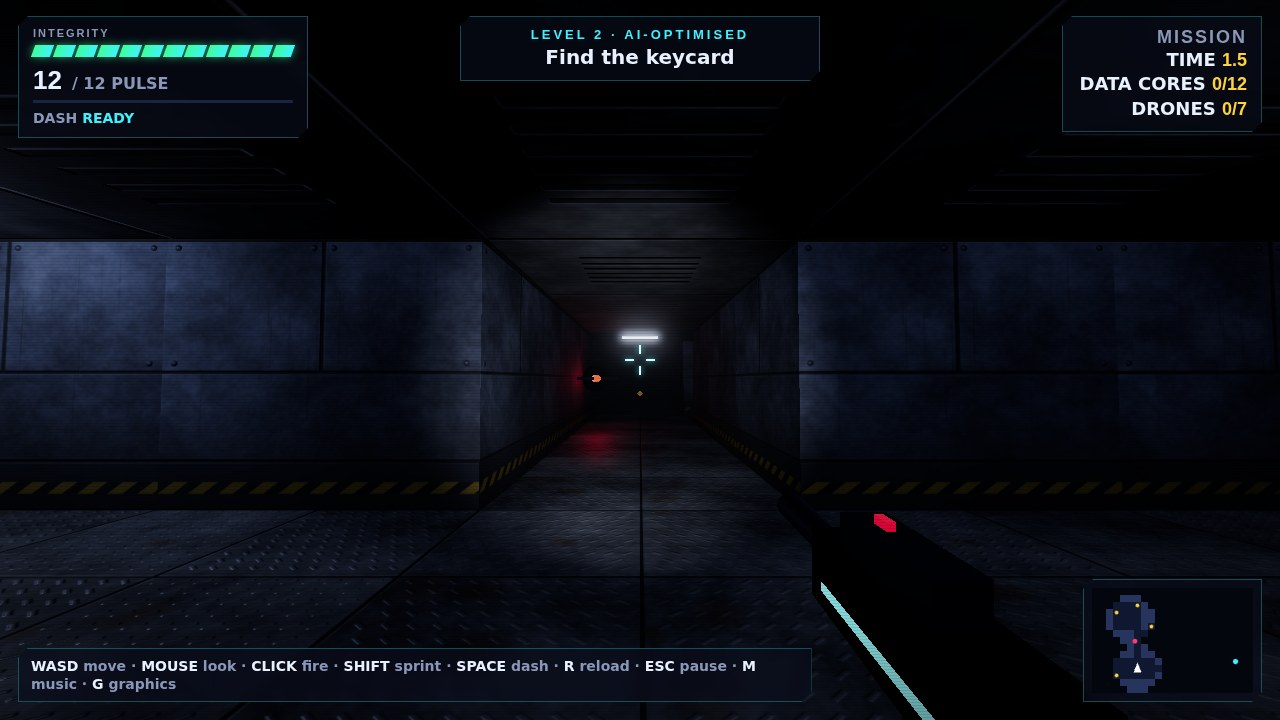
\includegraphics[width=\columnwidth]{fig_game.jpg}
\caption{\emph{LevelForge: Breach}, the playable first-person game built from the twin's levels
(level 2, the AI-optimised level). The twin's monsters appear as hunter drones (red, far end of the
corridor); the minimap at the bottom right shows the same grid as Fig.~\ref{fig:levels}.}
\label{fig:game}
\end{figure}

\subsection{Player Agents}
Each player agent plans with Dijkstra search over a persona-specific cost model, re-planning as the
level changes (picked-up items, defeated monsters). The \emph{rusher} pays almost nothing for danger,
the \emph{cautious} agent pays heavily for traps and monsters and detours to heal, and the
\emph{explorer} collects coins before exiting. Randomness in fights and traps comes from a seeded
generator, so each playthrough is defined by the tuple (level, persona, seed).

\subsection{Metrics and Quality Score}
For each level we aggregate completion, death and timeout rates, damage, backtracking ratio $\beta$
(steps that revisit tiles), exploration $x$, coin collection $\kappa$ by explorers, health lost by
finishers $h$, and completion per persona $c_p$. Five components in $[0,1]$ are
\begin{align*}
q_\text{bal} &= 1-\tfrac{|c-c^*|}{\max(c^*,1-c^*)}, &
q_\text{eng} &= 0.6\,\kappa + 0.4\min(1, x/0.6),\\
q_\text{flow} &= 1-2\beta, &
q_\text{skill} &= \tfrac{c_\text{cautious}-c_\text{rusher}}{0.35},\\
q_\text{ten} &= 1-\tfrac{|h-h^*|}{\max(h^*,1-h^*)}, &&
\end{align*}
each clipped to $[0,1]$, and the quality score is the weighted mean
$Q=\sum_k w_k q_k / \sum_k w_k$ with brief-derived weights. Balance penalises both under- and
overshooting the target; skill expression rewards levels where careful play beats reckless play.

\subsection{Design Agents and the Agent Loop}
The loop is a LangGraph~\cite{langgraph} state graph (Algorithm~\ref{alg:loop}).
The \textbf{generator} either loads the problem level supplied by the developer or asks the LLM to
write a grid from the brief; an invalid LLM grid gets one self-correction attempt, then
deterministic repair. The \textbf{critic} diagnoses the best level so far using a fixed vocabulary
of problem identifiers (e.g.\ \emph{too\_hard}, \emph{low\_skill\_expression}) and the metrics behind
them, and keeps a memory of priorities whose fixes were rejected, moving to a different priority
next time. The \textbf{optimizer} proposes $k=4$ alternative plans of structured edits: add or
remove a monster, trap, potion or coin on or off the main route; open a loop; add or remove a lock.
It also receives the simulated scores of the previous round's plans and which plans could not be
applied. The \textbf{finalizer} writes designer notes.

The LLM never edits the grid directly. Edits are validated and applied deterministically, so the
agents' reasoning is LLM-driven but every resulting level is guaranteed playable. The rule-based
variant replaces the LLM critic and optimizer with a hand-written diagnosis and playbook.

\begin{algorithm}[t]
\caption{Agent loop for one problem level}
\label{alg:loop}
\small
\begin{algorithmic}[1]
\Require level $L_0$ (or brief only), brief $B$, rounds $R$, plans $k$, runs $n$
\State $L^\star \gets$ \Call{Generator}{$L_0$, $B$};\quad $Q^\star \gets$ \Call{Simulate}{$\{L^\star\}$}
\State memory $\gets \emptyset$
\For{$r = 1$ to $R$}
  \State $D \gets$ \Call{Critic}{metrics$(L^\star)$, $B$, memory}
  \State $\{P_1..P_k\} \gets$ \Call{Optimizer}{$D$, last round's scores}
  \State $C_i \gets$ \Call{ApplyValidated}{$L^\star$, $P_i$} for $i=1..k$
  \State scores $\gets$ \Call{Simulate}{$\{C_1..C_k\}$} \Comment{$k \cdot 3n$ runs, parallel}
  \If{$\max_i Q(C_i) > Q^\star$}
     \State $L^\star, Q^\star \gets$ best candidate \Comment{accept}
  \Else
     \State memory $\gets$ memory $\cup \{D.\text{priority}\}$ \Comment{reject, roll back}
  \EndIf
\EndFor
\State \Return $L^\star$, \Call{Finalize}{history}
\end{algorithmic}
\end{algorithm}

\subsection{Parallel Play-Testing (Multicore)}
Every playthrough (level, persona, seed) is an independent task, so play-testing is embarrassingly
parallel: workers never communicate, and the only synchronisation is the final gather. In each
round the tasks of all $k$ candidates are combined into one sweep of $k\cdot 3n$ tasks over a
persistent process pool (default $p=5$). Processes are used instead of threads because the simulator
is CPU-bound Python and the global interpreter lock would serialise threads (review labelling, which
waits on the network, uses threads). The pool is created once per run, so its start-up cost is paid
once. All candidates use the same seeds (common random numbers~\cite{law2015simulation}), so score
differences come from the level, not from luck. Tasks are dispatched in small chunks (at most 8),
a choice based on the granularity study in Section~\ref{sec:scaling}.

\subsection{What the Developer Receives}
The goal is a level the developer can \emph{learn from}, not just a new grid. Each run produces an
HTML report with the review analysis, the score per round, every candidate the agents tried with its
score, the accepted plan per round, before/after levels, animated replays of each player agent, and
designer notes (Table~\ref{tab:case} is an excerpt). Finally, the levels are exported into the
playable 3D game, so the team can experience the problem level and its optimised version directly.
For the case study of Section~\ref{sec:case}, the notes read:

\begin{quote}
\small\itshape
``The initial level scored 0.48; after optimisation it scores 0.89. Completion moved from 32\% to
72\% against a review-derived target of 71\%. Backtracking went from 12\% to 4\% of steps, and
explorers now collect 100\% of the coins (was 77\%). Per-player-type completion (rusher / cautious /
explorer): 31\%/31\%/34\% $\to$ 66\%/100\%/51\%.''
\end{quote}

\noindent These notes come from the rule-based finalizer, which fills a template; the LLM
finalizer writes free-form notes that also explain \emph{why} each change helped.

\subsection{Implementation}
LevelForge is about 2,800 lines of Python. The agent loop uses LangGraph; parallel play-testing uses
the standard \texttt{multiprocessing} pool; the LLM client uses only the standard library and talks
to an OpenAI-compatible endpoint (Groq) in JSON mode, with retries that honour the server's
\texttt{Retry-After} header. If the API key is missing or a call fails permanently, every LLM step
falls back to its rule-based counterpart, so a demonstration cannot break mid-run. All randomness is
seeded, so runs are reproducible: for example,
\texttt{run\_demo.py --offline --level data/problem\_level.txt} reproduces the case study exactly.
The game is a single offline HTML file (Three.js bundled with esbuild) generated from the runs'
saved data, so it needs no server and no re-simulation.

% =====================================================================
\section{Experimental Setup}
% =====================================================================
\textbf{Hardware.} A laptop with \fillme{CPU model}, \fillme{N} physical cores and 12 logical
cores, \fillme{RAM} GB RAM, Windows, Python \fillme{version}. The GPU was not used for the
experiments.

\textbf{LLM.} GPT-OSS-120B~\cite{openai2025gptoss} served through the Groq API, with JSON output
mode and low reasoning effort. Every LLM step falls back to rules if a call fails.

\textbf{Optimisation study.} Since real reviewed levels were not available, 12 procedurally
generated levels serve as stand-ins for problem levels (their mean completion of 60\% is well below
the 71\% target). All methods start from the same level and get the same budget: 6 rounds $\times$ 4
candidates $\times$ 300 playthroughs. Methods: no optimisation (raw), random search (same loop with
random edits and no critic), and the agent loop with rule-based reasoning.

\textbf{LLM study.} The first 4 of those levels, adding the agent loop with LLM reasoning (99 API
calls, 425\,s in total). It is smaller because of free-tier API rate limits.

\textbf{Statistics.} Paired comparisons per level: exact two-sided Wilcoxon signed-rank
test~\cite{wilcoxon1945} and sign test.

\textbf{Scaling study.} 3,600 playthroughs (6 levels $\times$ 3 personas $\times$ 200) at 1--12
workers, best of 3 repeats, chunk size $n/(4p)$; then chunk sizes 1, 8, 180 and 720 at 5 workers.

% =====================================================================
\section{Results}
% =====================================================================
\subsection{Optimisation Quality}
Table~\ref{tab:main} summarises the 12-level study. Both optimisers improved every level over the
raw level (Wilcoxon $p<0.001$ each): $+32\%$ for random search and $+37\%$ for the agent loop. The
agent loop beat random search on 9 of 12 levels, with a mean paired gain of $+0.026$ (Wilcoxon
$p=0.034$). The sign test is weaker ($p=0.146$) because it ignores the size of each difference: the
agent's wins (up to $+0.089$) were larger than its losses (at most $-0.020$). The agent loop also
landed closer to the completion target (74\% vs.\ 78\%).

\begin{table}[t]
\caption{Optimisation quality on 12 levels (same budget; completion target 71\%)}
\label{tab:main}
\centering
\footnotesize
\begin{tabular}{@{}lcc@{}}
\toprule
Method & $Q$ (mean $\pm$ sd) & Completion \\
\midrule
No optimisation (raw) & $0.572 \pm 0.093$ & 60\% \\
Random search & $0.758 \pm 0.064$ & 78\% \\
Agent loop, rule-based & $\mathbf{0.783 \pm 0.061}$ & 74\% \\
\bottomrule
\end{tabular}
\end{table}

Fig.~\ref{fig:conv} shows the best quality per round. The agent loop reached random search's final
quality (0.758) by round 4, i.e.\ with about two thirds of the simulation budget.

\begin{figure}[t]
\centering
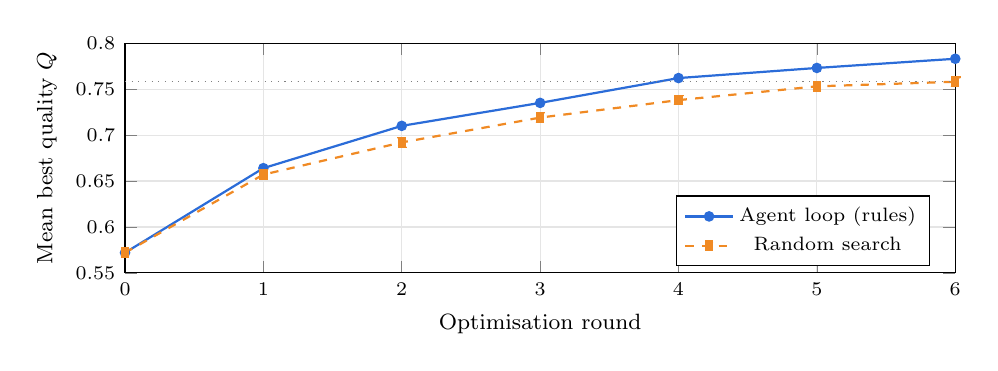
\begin{tikzpicture}
\begin{axis}[
  width=\columnwidth, height=45mm,
  xlabel={Optimisation round}, ylabel={Mean best quality $Q$},
  xmin=0, xmax=6, ymin=0.55, ymax=0.80,
  xtick={0,...,6}, ytick={0.55,0.60,...,0.80},
  yticklabel style={/pgf/number format/fixed, /pgf/number format/precision=2},
  grid=major, grid style={gray!20},
  legend pos=south east, legend style={font=\scriptsize},
  tick label style={font=\scriptsize}, label style={font=\footnotesize},
]
\addplot[thick, color=lfexit, mark=*, mark size=1.5pt] coordinates
  {(0,0.572)(1,0.664)(2,0.710)(3,0.735)(4,0.762)(5,0.773)(6,0.783)};
\addlegendentry{Agent loop (rules)}
\addplot[thick, dashed, color=lftrap, mark=square*, mark size=1.5pt] coordinates
  {(0,0.572)(1,0.657)(2,0.692)(3,0.719)(4,0.738)(5,0.753)(6,0.758)};
\addlegendentry{Random search}
\addplot[thin, gray, dotted, domain=0:6] {0.758};
\end{axis}
\end{tikzpicture}
\caption{Convergence over 12 levels. The dotted line is random search's final quality, which the
agent loop reaches by round 4.}
\label{fig:conv}
\end{figure}

\subsection{LLM vs.\ Rule-Based Design Agents}
On the 4-level subset (Table~\ref{tab:llm}) the LLM agent won 2 of 4 levels against random search
and 2 of 4 against the rule-based agent. With 4 levels no difference is statistically detectable
(the smallest possible two-sided sign test $p$-value is 0.125), so we report the methods as
comparable. The LLM agent had the highest variance: the best result on two levels (0.804, 0.844)
and the worst agent result on another (0.655).

\begin{table}[t]
\caption{LLM vs.\ rule-based reasoning (4 levels)}
\label{tab:llm}
\centering
\footnotesize
\begin{tabular}{@{}lc@{}}
\toprule
Method & Quality $Q$ (mean $\pm$ sd) \\
\midrule
No optimisation (raw) & $0.631 \pm 0.012$ \\
Random search & $0.757 \pm 0.053$ \\
Agent loop, rule-based & $\mathbf{0.787 \pm 0.026}$ \\
Agent loop, LLM (GPT-OSS-120B) & $0.766 \pm 0.082$ \\
\bottomrule
\end{tabular}
\end{table}

\subsection{Case Study: Repairing a Problem Level}
\label{sec:case}
Fig.~\ref{fig:levels} shows a problem level before and after optimisation, and Table~\ref{tab:case}
shows what the developer sees round by round. Only 32\% of playthroughs reached the exit (target
71\%) and, worse for design, reckless and careful players did equally badly (31\% vs.\ 31\%), so
skill was not rewarded. After six rounds and 11,250 simulated playthroughs (19\,s on 2 workers),
quality rose from 0.477 to 0.895: completion 72\%, backtracking down from 12\% to 4\% of steps, and
per-persona completion (rusher/cautious/explorer) changed from 31/31/34\% to 66/100/51\%, so careful
play now pays off. Only 12 tiles changed, which makes the fix easy for a designer to review. The
component scores moved as follows: balance 0.45$\to$0.98, engagement 0.62$\to$0.86, flow
0.77$\to$0.92, skill 0.02$\to$0.97 and tension 0.42$\to$0.63; tension improved least, because
finishers still lose 59\% of their health against a target of 35\%. Fig.~\ref{fig:persona}
shows the per-persona effect, which is the part of the result a designer is most likely to act on.

\begin{figure}[t]
\centering
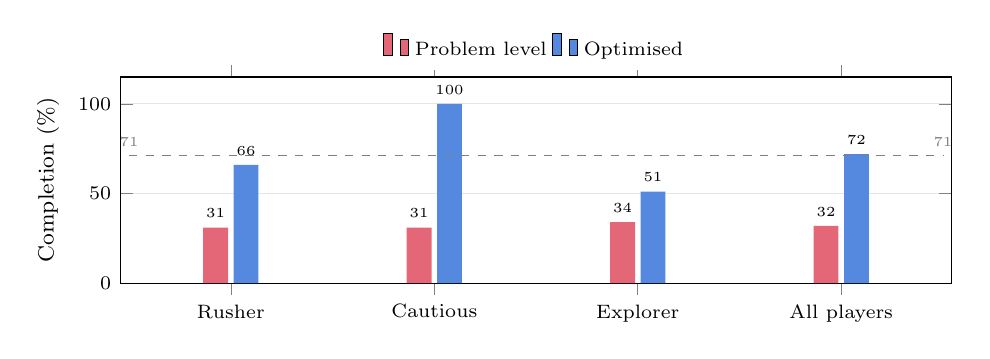
\begin{tikzpicture}
\begin{axis}[
  ybar, bar width=9pt, width=\columnwidth, height=42mm,
  ymin=0, ymax=115, ylabel={Completion (\%)},
  symbolic x coords={Rusher,Cautious,Explorer,All players}, xtick=data,
  nodes near coords, nodes near coords style={font=\tiny},
  enlarge x limits=0.18,
  legend style={font=\scriptsize, at={(0.5,1.03)}, anchor=south, legend columns=2, draw=none},
  tick label style={font=\scriptsize}, label style={font=\footnotesize},
  ymajorgrids, grid style={gray!20},
]
\addplot[fill=lfmon!70, draw=none] coordinates {(Rusher,31) (Cautious,31) (Explorer,34) (All players,32)};
\addlegendentry{Problem level}
\addplot[fill=lfexit!80, draw=none] coordinates {(Rusher,66) (Cautious,100) (Explorer,51) (All players,72)};
\addlegendentry{Optimised}
\addplot[thin, dashed, gray, sharp plot, update limits=false] coordinates {([normalized]-0.5,71) ([normalized]3.5,71)};
\end{axis}
\end{tikzpicture}
\caption{Completion per player agent in the case study. Before optimisation all play styles did
equally badly, so skill did not matter; afterwards careful play is rewarded and overall completion
is close to the review-derived target (dashed, 71\%).}
\label{fig:persona}
\end{figure}

\begin{figure}[t]
\centering
% generated from data/problem_level.txt and the optimised level of the same run
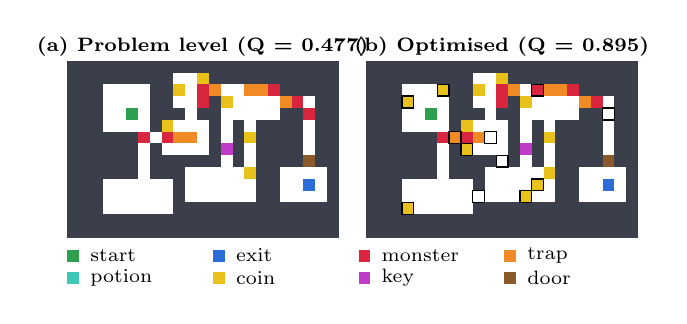
\begin{tikzpicture}
\fill[lfwall] (0.00,2.10) rectangle ++(0.15,0.15);
\fill[lfwall] (0.15,2.10) rectangle ++(0.15,0.15);
\fill[lfwall] (0.30,2.10) rectangle ++(0.15,0.15);
\fill[lfwall] (0.45,2.10) rectangle ++(0.15,0.15);
\fill[lfwall] (0.60,2.10) rectangle ++(0.15,0.15);
\fill[lfwall] (0.75,2.10) rectangle ++(0.15,0.15);
\fill[lfwall] (0.90,2.10) rectangle ++(0.15,0.15);
\fill[lfwall] (1.05,2.10) rectangle ++(0.15,0.15);
\fill[lfwall] (1.20,2.10) rectangle ++(0.15,0.15);
\fill[lfwall] (1.35,2.10) rectangle ++(0.15,0.15);
\fill[lfwall] (1.50,2.10) rectangle ++(0.15,0.15);
\fill[lfwall] (1.65,2.10) rectangle ++(0.15,0.15);
\fill[lfwall] (1.80,2.10) rectangle ++(0.15,0.15);
\fill[lfwall] (1.95,2.10) rectangle ++(0.15,0.15);
\fill[lfwall] (2.10,2.10) rectangle ++(0.15,0.15);
\fill[lfwall] (2.25,2.10) rectangle ++(0.15,0.15);
\fill[lfwall] (2.40,2.10) rectangle ++(0.15,0.15);
\fill[lfwall] (2.55,2.10) rectangle ++(0.15,0.15);
\fill[lfwall] (2.70,2.10) rectangle ++(0.15,0.15);
\fill[lfwall] (2.85,2.10) rectangle ++(0.15,0.15);
\fill[lfwall] (3.00,2.10) rectangle ++(0.15,0.15);
\fill[lfwall] (3.15,2.10) rectangle ++(0.15,0.15);
\fill[lfwall] (3.30,2.10) rectangle ++(0.15,0.15);
\fill[lfwall] (0.00,1.95) rectangle ++(0.15,0.15);
\fill[lfwall] (0.15,1.95) rectangle ++(0.15,0.15);
\fill[lfwall] (0.30,1.95) rectangle ++(0.15,0.15);
\fill[lfwall] (0.45,1.95) rectangle ++(0.15,0.15);
\fill[lfwall] (0.60,1.95) rectangle ++(0.15,0.15);
\fill[lfwall] (0.75,1.95) rectangle ++(0.15,0.15);
\fill[lfwall] (0.90,1.95) rectangle ++(0.15,0.15);
\fill[lfwall] (1.05,1.95) rectangle ++(0.15,0.15);
\fill[lfwall] (1.20,1.95) rectangle ++(0.15,0.15);
\fill[white] (1.35,1.95) rectangle ++(0.15,0.15);
\fill[white] (1.50,1.95) rectangle ++(0.15,0.15);
\fill[lfcoin] (1.65,1.95) rectangle ++(0.15,0.15);
\fill[lfwall] (1.80,1.95) rectangle ++(0.15,0.15);
\fill[lfwall] (1.95,1.95) rectangle ++(0.15,0.15);
\fill[lfwall] (2.10,1.95) rectangle ++(0.15,0.15);
\fill[lfwall] (2.25,1.95) rectangle ++(0.15,0.15);
\fill[lfwall] (2.40,1.95) rectangle ++(0.15,0.15);
\fill[lfwall] (2.55,1.95) rectangle ++(0.15,0.15);
\fill[lfwall] (2.70,1.95) rectangle ++(0.15,0.15);
\fill[lfwall] (2.85,1.95) rectangle ++(0.15,0.15);
\fill[lfwall] (3.00,1.95) rectangle ++(0.15,0.15);
\fill[lfwall] (3.15,1.95) rectangle ++(0.15,0.15);
\fill[lfwall] (3.30,1.95) rectangle ++(0.15,0.15);
\fill[lfwall] (0.00,1.80) rectangle ++(0.15,0.15);
\fill[lfwall] (0.15,1.80) rectangle ++(0.15,0.15);
\fill[lfwall] (0.30,1.80) rectangle ++(0.15,0.15);
\fill[white] (0.45,1.80) rectangle ++(0.15,0.15);
\fill[white] (0.60,1.80) rectangle ++(0.15,0.15);
\fill[white] (0.75,1.80) rectangle ++(0.15,0.15);
\fill[white] (0.90,1.80) rectangle ++(0.15,0.15);
\fill[lfwall] (1.05,1.80) rectangle ++(0.15,0.15);
\fill[lfwall] (1.20,1.80) rectangle ++(0.15,0.15);
\fill[lfcoin] (1.35,1.80) rectangle ++(0.15,0.15);
\fill[white] (1.50,1.80) rectangle ++(0.15,0.15);
\fill[lfmon] (1.65,1.80) rectangle ++(0.15,0.15);
\fill[lftrap] (1.80,1.80) rectangle ++(0.15,0.15);
\fill[white] (1.95,1.80) rectangle ++(0.15,0.15);
\fill[white] (2.10,1.80) rectangle ++(0.15,0.15);
\fill[lftrap] (2.25,1.80) rectangle ++(0.15,0.15);
\fill[lftrap] (2.40,1.80) rectangle ++(0.15,0.15);
\fill[lfmon] (2.55,1.80) rectangle ++(0.15,0.15);
\fill[lfwall] (2.70,1.80) rectangle ++(0.15,0.15);
\fill[lfwall] (2.85,1.80) rectangle ++(0.15,0.15);
\fill[lfwall] (3.00,1.80) rectangle ++(0.15,0.15);
\fill[lfwall] (3.15,1.80) rectangle ++(0.15,0.15);
\fill[lfwall] (3.30,1.80) rectangle ++(0.15,0.15);
\fill[lfwall] (0.00,1.65) rectangle ++(0.15,0.15);
\fill[lfwall] (0.15,1.65) rectangle ++(0.15,0.15);
\fill[lfwall] (0.30,1.65) rectangle ++(0.15,0.15);
\fill[white] (0.45,1.65) rectangle ++(0.15,0.15);
\fill[white] (0.60,1.65) rectangle ++(0.15,0.15);
\fill[white] (0.75,1.65) rectangle ++(0.15,0.15);
\fill[white] (0.90,1.65) rectangle ++(0.15,0.15);
\fill[lfwall] (1.05,1.65) rectangle ++(0.15,0.15);
\fill[lfwall] (1.20,1.65) rectangle ++(0.15,0.15);
\fill[white] (1.35,1.65) rectangle ++(0.15,0.15);
\fill[white] (1.50,1.65) rectangle ++(0.15,0.15);
\fill[lfmon] (1.65,1.65) rectangle ++(0.15,0.15);
\fill[lfwall] (1.80,1.65) rectangle ++(0.15,0.15);
\fill[lfcoin] (1.95,1.65) rectangle ++(0.15,0.15);
\fill[white] (2.10,1.65) rectangle ++(0.15,0.15);
\fill[white] (2.25,1.65) rectangle ++(0.15,0.15);
\fill[white] (2.40,1.65) rectangle ++(0.15,0.15);
\fill[white] (2.55,1.65) rectangle ++(0.15,0.15);
\fill[lftrap] (2.70,1.65) rectangle ++(0.15,0.15);
\fill[lfmon] (2.85,1.65) rectangle ++(0.15,0.15);
\fill[white] (3.00,1.65) rectangle ++(0.15,0.15);
\fill[lfwall] (3.15,1.65) rectangle ++(0.15,0.15);
\fill[lfwall] (3.30,1.65) rectangle ++(0.15,0.15);
\fill[lfwall] (0.00,1.50) rectangle ++(0.15,0.15);
\fill[lfwall] (0.15,1.50) rectangle ++(0.15,0.15);
\fill[lfwall] (0.30,1.50) rectangle ++(0.15,0.15);
\fill[white] (0.45,1.50) rectangle ++(0.15,0.15);
\fill[white] (0.60,1.50) rectangle ++(0.15,0.15);
\fill[lfstart] (0.75,1.50) rectangle ++(0.15,0.15);
\fill[white] (0.90,1.50) rectangle ++(0.15,0.15);
\fill[lfwall] (1.05,1.50) rectangle ++(0.15,0.15);
\fill[lfwall] (1.20,1.50) rectangle ++(0.15,0.15);
\fill[lfwall] (1.35,1.50) rectangle ++(0.15,0.15);
\fill[white] (1.50,1.50) rectangle ++(0.15,0.15);
\fill[lfwall] (1.65,1.50) rectangle ++(0.15,0.15);
\fill[lfwall] (1.80,1.50) rectangle ++(0.15,0.15);
\fill[white] (1.95,1.50) rectangle ++(0.15,0.15);
\fill[white] (2.10,1.50) rectangle ++(0.15,0.15);
\fill[white] (2.25,1.50) rectangle ++(0.15,0.15);
\fill[white] (2.40,1.50) rectangle ++(0.15,0.15);
\fill[white] (2.55,1.50) rectangle ++(0.15,0.15);
\fill[lfwall] (2.70,1.50) rectangle ++(0.15,0.15);
\fill[lfwall] (2.85,1.50) rectangle ++(0.15,0.15);
\fill[lfmon] (3.00,1.50) rectangle ++(0.15,0.15);
\fill[lfwall] (3.15,1.50) rectangle ++(0.15,0.15);
\fill[lfwall] (3.30,1.50) rectangle ++(0.15,0.15);
\fill[lfwall] (0.00,1.35) rectangle ++(0.15,0.15);
\fill[lfwall] (0.15,1.35) rectangle ++(0.15,0.15);
\fill[lfwall] (0.30,1.35) rectangle ++(0.15,0.15);
\fill[white] (0.45,1.35) rectangle ++(0.15,0.15);
\fill[white] (0.60,1.35) rectangle ++(0.15,0.15);
\fill[white] (0.75,1.35) rectangle ++(0.15,0.15);
\fill[white] (0.90,1.35) rectangle ++(0.15,0.15);
\fill[lfwall] (1.05,1.35) rectangle ++(0.15,0.15);
\fill[lfcoin] (1.20,1.35) rectangle ++(0.15,0.15);
\fill[white] (1.35,1.35) rectangle ++(0.15,0.15);
\fill[white] (1.50,1.35) rectangle ++(0.15,0.15);
\fill[white] (1.65,1.35) rectangle ++(0.15,0.15);
\fill[lfwall] (1.80,1.35) rectangle ++(0.15,0.15);
\fill[white] (1.95,1.35) rectangle ++(0.15,0.15);
\fill[lfwall] (2.10,1.35) rectangle ++(0.15,0.15);
\fill[white] (2.25,1.35) rectangle ++(0.15,0.15);
\fill[lfwall] (2.40,1.35) rectangle ++(0.15,0.15);
\fill[lfwall] (2.55,1.35) rectangle ++(0.15,0.15);
\fill[lfwall] (2.70,1.35) rectangle ++(0.15,0.15);
\fill[lfwall] (2.85,1.35) rectangle ++(0.15,0.15);
\fill[white] (3.00,1.35) rectangle ++(0.15,0.15);
\fill[lfwall] (3.15,1.35) rectangle ++(0.15,0.15);
\fill[lfwall] (3.30,1.35) rectangle ++(0.15,0.15);
\fill[lfwall] (0.00,1.20) rectangle ++(0.15,0.15);
\fill[lfwall] (0.15,1.20) rectangle ++(0.15,0.15);
\fill[lfwall] (0.30,1.20) rectangle ++(0.15,0.15);
\fill[lfwall] (0.45,1.20) rectangle ++(0.15,0.15);
\fill[lfwall] (0.60,1.20) rectangle ++(0.15,0.15);
\fill[lfwall] (0.75,1.20) rectangle ++(0.15,0.15);
\fill[lfmon] (0.90,1.20) rectangle ++(0.15,0.15);
\fill[white] (1.05,1.20) rectangle ++(0.15,0.15);
\fill[lfmon] (1.20,1.20) rectangle ++(0.15,0.15);
\fill[lftrap] (1.35,1.20) rectangle ++(0.15,0.15);
\fill[lftrap] (1.50,1.20) rectangle ++(0.15,0.15);
\fill[white] (1.65,1.20) rectangle ++(0.15,0.15);
\fill[lfwall] (1.80,1.20) rectangle ++(0.15,0.15);
\fill[white] (1.95,1.20) rectangle ++(0.15,0.15);
\fill[lfwall] (2.10,1.20) rectangle ++(0.15,0.15);
\fill[lfcoin] (2.25,1.20) rectangle ++(0.15,0.15);
\fill[lfwall] (2.40,1.20) rectangle ++(0.15,0.15);
\fill[lfwall] (2.55,1.20) rectangle ++(0.15,0.15);
\fill[lfwall] (2.70,1.20) rectangle ++(0.15,0.15);
\fill[lfwall] (2.85,1.20) rectangle ++(0.15,0.15);
\fill[white] (3.00,1.20) rectangle ++(0.15,0.15);
\fill[lfwall] (3.15,1.20) rectangle ++(0.15,0.15);
\fill[lfwall] (3.30,1.20) rectangle ++(0.15,0.15);
\fill[lfwall] (0.00,1.05) rectangle ++(0.15,0.15);
\fill[lfwall] (0.15,1.05) rectangle ++(0.15,0.15);
\fill[lfwall] (0.30,1.05) rectangle ++(0.15,0.15);
\fill[lfwall] (0.45,1.05) rectangle ++(0.15,0.15);
\fill[lfwall] (0.60,1.05) rectangle ++(0.15,0.15);
\fill[lfwall] (0.75,1.05) rectangle ++(0.15,0.15);
\fill[white] (0.90,1.05) rectangle ++(0.15,0.15);
\fill[lfwall] (1.05,1.05) rectangle ++(0.15,0.15);
\fill[white] (1.20,1.05) rectangle ++(0.15,0.15);
\fill[white] (1.35,1.05) rectangle ++(0.15,0.15);
\fill[white] (1.50,1.05) rectangle ++(0.15,0.15);
\fill[white] (1.65,1.05) rectangle ++(0.15,0.15);
\fill[lfwall] (1.80,1.05) rectangle ++(0.15,0.15);
\fill[lfkey] (1.95,1.05) rectangle ++(0.15,0.15);
\fill[lfwall] (2.10,1.05) rectangle ++(0.15,0.15);
\fill[white] (2.25,1.05) rectangle ++(0.15,0.15);
\fill[lfwall] (2.40,1.05) rectangle ++(0.15,0.15);
\fill[lfwall] (2.55,1.05) rectangle ++(0.15,0.15);
\fill[lfwall] (2.70,1.05) rectangle ++(0.15,0.15);
\fill[lfwall] (2.85,1.05) rectangle ++(0.15,0.15);
\fill[white] (3.00,1.05) rectangle ++(0.15,0.15);
\fill[lfwall] (3.15,1.05) rectangle ++(0.15,0.15);
\fill[lfwall] (3.30,1.05) rectangle ++(0.15,0.15);
\fill[lfwall] (0.00,0.90) rectangle ++(0.15,0.15);
\fill[lfwall] (0.15,0.90) rectangle ++(0.15,0.15);
\fill[lfwall] (0.30,0.90) rectangle ++(0.15,0.15);
\fill[lfwall] (0.45,0.90) rectangle ++(0.15,0.15);
\fill[lfwall] (0.60,0.90) rectangle ++(0.15,0.15);
\fill[lfwall] (0.75,0.90) rectangle ++(0.15,0.15);
\fill[white] (0.90,0.90) rectangle ++(0.15,0.15);
\fill[lfwall] (1.05,0.90) rectangle ++(0.15,0.15);
\fill[lfwall] (1.20,0.90) rectangle ++(0.15,0.15);
\fill[lfwall] (1.35,0.90) rectangle ++(0.15,0.15);
\fill[lfwall] (1.50,0.90) rectangle ++(0.15,0.15);
\fill[lfwall] (1.65,0.90) rectangle ++(0.15,0.15);
\fill[lfwall] (1.80,0.90) rectangle ++(0.15,0.15);
\fill[white] (1.95,0.90) rectangle ++(0.15,0.15);
\fill[lfwall] (2.10,0.90) rectangle ++(0.15,0.15);
\fill[white] (2.25,0.90) rectangle ++(0.15,0.15);
\fill[lfwall] (2.40,0.90) rectangle ++(0.15,0.15);
\fill[lfwall] (2.55,0.90) rectangle ++(0.15,0.15);
\fill[lfwall] (2.70,0.90) rectangle ++(0.15,0.15);
\fill[lfwall] (2.85,0.90) rectangle ++(0.15,0.15);
\fill[lfdoor] (3.00,0.90) rectangle ++(0.15,0.15);
\fill[lfwall] (3.15,0.90) rectangle ++(0.15,0.15);
\fill[lfwall] (3.30,0.90) rectangle ++(0.15,0.15);
\fill[lfwall] (0.00,0.75) rectangle ++(0.15,0.15);
\fill[lfwall] (0.15,0.75) rectangle ++(0.15,0.15);
\fill[lfwall] (0.30,0.75) rectangle ++(0.15,0.15);
\fill[lfwall] (0.45,0.75) rectangle ++(0.15,0.15);
\fill[lfwall] (0.60,0.75) rectangle ++(0.15,0.15);
\fill[lfwall] (0.75,0.75) rectangle ++(0.15,0.15);
\fill[white] (0.90,0.75) rectangle ++(0.15,0.15);
\fill[lfwall] (1.05,0.75) rectangle ++(0.15,0.15);
\fill[lfwall] (1.20,0.75) rectangle ++(0.15,0.15);
\fill[lfwall] (1.35,0.75) rectangle ++(0.15,0.15);
\fill[white] (1.50,0.75) rectangle ++(0.15,0.15);
\fill[white] (1.65,0.75) rectangle ++(0.15,0.15);
\fill[white] (1.80,0.75) rectangle ++(0.15,0.15);
\fill[white] (1.95,0.75) rectangle ++(0.15,0.15);
\fill[white] (2.10,0.75) rectangle ++(0.15,0.15);
\fill[lfcoin] (2.25,0.75) rectangle ++(0.15,0.15);
\fill[lfwall] (2.40,0.75) rectangle ++(0.15,0.15);
\fill[lfwall] (2.55,0.75) rectangle ++(0.15,0.15);
\fill[white] (2.70,0.75) rectangle ++(0.15,0.15);
\fill[white] (2.85,0.75) rectangle ++(0.15,0.15);
\fill[white] (3.00,0.75) rectangle ++(0.15,0.15);
\fill[white] (3.15,0.75) rectangle ++(0.15,0.15);
\fill[lfwall] (3.30,0.75) rectangle ++(0.15,0.15);
\fill[lfwall] (0.00,0.60) rectangle ++(0.15,0.15);
\fill[lfwall] (0.15,0.60) rectangle ++(0.15,0.15);
\fill[lfwall] (0.30,0.60) rectangle ++(0.15,0.15);
\fill[white] (0.45,0.60) rectangle ++(0.15,0.15);
\fill[white] (0.60,0.60) rectangle ++(0.15,0.15);
\fill[white] (0.75,0.60) rectangle ++(0.15,0.15);
\fill[white] (0.90,0.60) rectangle ++(0.15,0.15);
\fill[white] (1.05,0.60) rectangle ++(0.15,0.15);
\fill[white] (1.20,0.60) rectangle ++(0.15,0.15);
\fill[lfwall] (1.35,0.60) rectangle ++(0.15,0.15);
\fill[white] (1.50,0.60) rectangle ++(0.15,0.15);
\fill[white] (1.65,0.60) rectangle ++(0.15,0.15);
\fill[white] (1.80,0.60) rectangle ++(0.15,0.15);
\fill[white] (1.95,0.60) rectangle ++(0.15,0.15);
\fill[white] (2.10,0.60) rectangle ++(0.15,0.15);
\fill[white] (2.25,0.60) rectangle ++(0.15,0.15);
\fill[lfwall] (2.40,0.60) rectangle ++(0.15,0.15);
\fill[lfwall] (2.55,0.60) rectangle ++(0.15,0.15);
\fill[white] (2.70,0.60) rectangle ++(0.15,0.15);
\fill[white] (2.85,0.60) rectangle ++(0.15,0.15);
\fill[lfexit] (3.00,0.60) rectangle ++(0.15,0.15);
\fill[white] (3.15,0.60) rectangle ++(0.15,0.15);
\fill[lfwall] (3.30,0.60) rectangle ++(0.15,0.15);
\fill[lfwall] (0.00,0.45) rectangle ++(0.15,0.15);
\fill[lfwall] (0.15,0.45) rectangle ++(0.15,0.15);
\fill[lfwall] (0.30,0.45) rectangle ++(0.15,0.15);
\fill[white] (0.45,0.45) rectangle ++(0.15,0.15);
\fill[white] (0.60,0.45) rectangle ++(0.15,0.15);
\fill[white] (0.75,0.45) rectangle ++(0.15,0.15);
\fill[white] (0.90,0.45) rectangle ++(0.15,0.15);
\fill[white] (1.05,0.45) rectangle ++(0.15,0.15);
\fill[white] (1.20,0.45) rectangle ++(0.15,0.15);
\fill[lfwall] (1.35,0.45) rectangle ++(0.15,0.15);
\fill[white] (1.50,0.45) rectangle ++(0.15,0.15);
\fill[white] (1.65,0.45) rectangle ++(0.15,0.15);
\fill[white] (1.80,0.45) rectangle ++(0.15,0.15);
\fill[white] (1.95,0.45) rectangle ++(0.15,0.15);
\fill[white] (2.10,0.45) rectangle ++(0.15,0.15);
\fill[white] (2.25,0.45) rectangle ++(0.15,0.15);
\fill[lfwall] (2.40,0.45) rectangle ++(0.15,0.15);
\fill[lfwall] (2.55,0.45) rectangle ++(0.15,0.15);
\fill[white] (2.70,0.45) rectangle ++(0.15,0.15);
\fill[white] (2.85,0.45) rectangle ++(0.15,0.15);
\fill[white] (3.00,0.45) rectangle ++(0.15,0.15);
\fill[white] (3.15,0.45) rectangle ++(0.15,0.15);
\fill[lfwall] (3.30,0.45) rectangle ++(0.15,0.15);
\fill[lfwall] (0.00,0.30) rectangle ++(0.15,0.15);
\fill[lfwall] (0.15,0.30) rectangle ++(0.15,0.15);
\fill[lfwall] (0.30,0.30) rectangle ++(0.15,0.15);
\fill[white] (0.45,0.30) rectangle ++(0.15,0.15);
\fill[white] (0.60,0.30) rectangle ++(0.15,0.15);
\fill[white] (0.75,0.30) rectangle ++(0.15,0.15);
\fill[white] (0.90,0.30) rectangle ++(0.15,0.15);
\fill[white] (1.05,0.30) rectangle ++(0.15,0.15);
\fill[white] (1.20,0.30) rectangle ++(0.15,0.15);
\fill[lfwall] (1.35,0.30) rectangle ++(0.15,0.15);
\fill[lfwall] (1.50,0.30) rectangle ++(0.15,0.15);
\fill[lfwall] (1.65,0.30) rectangle ++(0.15,0.15);
\fill[lfwall] (1.80,0.30) rectangle ++(0.15,0.15);
\fill[lfwall] (1.95,0.30) rectangle ++(0.15,0.15);
\fill[lfwall] (2.10,0.30) rectangle ++(0.15,0.15);
\fill[lfwall] (2.25,0.30) rectangle ++(0.15,0.15);
\fill[lfwall] (2.40,0.30) rectangle ++(0.15,0.15);
\fill[lfwall] (2.55,0.30) rectangle ++(0.15,0.15);
\fill[lfwall] (2.70,0.30) rectangle ++(0.15,0.15);
\fill[lfwall] (2.85,0.30) rectangle ++(0.15,0.15);
\fill[lfwall] (3.00,0.30) rectangle ++(0.15,0.15);
\fill[lfwall] (3.15,0.30) rectangle ++(0.15,0.15);
\fill[lfwall] (3.30,0.30) rectangle ++(0.15,0.15);
\fill[lfwall] (0.00,0.15) rectangle ++(0.15,0.15);
\fill[lfwall] (0.15,0.15) rectangle ++(0.15,0.15);
\fill[lfwall] (0.30,0.15) rectangle ++(0.15,0.15);
\fill[lfwall] (0.45,0.15) rectangle ++(0.15,0.15);
\fill[lfwall] (0.60,0.15) rectangle ++(0.15,0.15);
\fill[lfwall] (0.75,0.15) rectangle ++(0.15,0.15);
\fill[lfwall] (0.90,0.15) rectangle ++(0.15,0.15);
\fill[lfwall] (1.05,0.15) rectangle ++(0.15,0.15);
\fill[lfwall] (1.20,0.15) rectangle ++(0.15,0.15);
\fill[lfwall] (1.35,0.15) rectangle ++(0.15,0.15);
\fill[lfwall] (1.50,0.15) rectangle ++(0.15,0.15);
\fill[lfwall] (1.65,0.15) rectangle ++(0.15,0.15);
\fill[lfwall] (1.80,0.15) rectangle ++(0.15,0.15);
\fill[lfwall] (1.95,0.15) rectangle ++(0.15,0.15);
\fill[lfwall] (2.10,0.15) rectangle ++(0.15,0.15);
\fill[lfwall] (2.25,0.15) rectangle ++(0.15,0.15);
\fill[lfwall] (2.40,0.15) rectangle ++(0.15,0.15);
\fill[lfwall] (2.55,0.15) rectangle ++(0.15,0.15);
\fill[lfwall] (2.70,0.15) rectangle ++(0.15,0.15);
\fill[lfwall] (2.85,0.15) rectangle ++(0.15,0.15);
\fill[lfwall] (3.00,0.15) rectangle ++(0.15,0.15);
\fill[lfwall] (3.15,0.15) rectangle ++(0.15,0.15);
\fill[lfwall] (3.30,0.15) rectangle ++(0.15,0.15);
\fill[lfwall] (0.00,0.00) rectangle ++(0.15,0.15);
\fill[lfwall] (0.15,0.00) rectangle ++(0.15,0.15);
\fill[lfwall] (0.30,0.00) rectangle ++(0.15,0.15);
\fill[lfwall] (0.45,0.00) rectangle ++(0.15,0.15);
\fill[lfwall] (0.60,0.00) rectangle ++(0.15,0.15);
\fill[lfwall] (0.75,0.00) rectangle ++(0.15,0.15);
\fill[lfwall] (0.90,0.00) rectangle ++(0.15,0.15);
\fill[lfwall] (1.05,0.00) rectangle ++(0.15,0.15);
\fill[lfwall] (1.20,0.00) rectangle ++(0.15,0.15);
\fill[lfwall] (1.35,0.00) rectangle ++(0.15,0.15);
\fill[lfwall] (1.50,0.00) rectangle ++(0.15,0.15);
\fill[lfwall] (1.65,0.00) rectangle ++(0.15,0.15);
\fill[lfwall] (1.80,0.00) rectangle ++(0.15,0.15);
\fill[lfwall] (1.95,0.00) rectangle ++(0.15,0.15);
\fill[lfwall] (2.10,0.00) rectangle ++(0.15,0.15);
\fill[lfwall] (2.25,0.00) rectangle ++(0.15,0.15);
\fill[lfwall] (2.40,0.00) rectangle ++(0.15,0.15);
\fill[lfwall] (2.55,0.00) rectangle ++(0.15,0.15);
\fill[lfwall] (2.70,0.00) rectangle ++(0.15,0.15);
\fill[lfwall] (2.85,0.00) rectangle ++(0.15,0.15);
\fill[lfwall] (3.00,0.00) rectangle ++(0.15,0.15);
\fill[lfwall] (3.15,0.00) rectangle ++(0.15,0.15);
\fill[lfwall] (3.30,0.00) rectangle ++(0.15,0.15);
\fill[lfwall] (3.80,2.10) rectangle ++(0.15,0.15);
\fill[lfwall] (3.95,2.10) rectangle ++(0.15,0.15);
\fill[lfwall] (4.10,2.10) rectangle ++(0.15,0.15);
\fill[lfwall] (4.25,2.10) rectangle ++(0.15,0.15);
\fill[lfwall] (4.40,2.10) rectangle ++(0.15,0.15);
\fill[lfwall] (4.55,2.10) rectangle ++(0.15,0.15);
\fill[lfwall] (4.70,2.10) rectangle ++(0.15,0.15);
\fill[lfwall] (4.85,2.10) rectangle ++(0.15,0.15);
\fill[lfwall] (5.00,2.10) rectangle ++(0.15,0.15);
\fill[lfwall] (5.15,2.10) rectangle ++(0.15,0.15);
\fill[lfwall] (5.30,2.10) rectangle ++(0.15,0.15);
\fill[lfwall] (5.45,2.10) rectangle ++(0.15,0.15);
\fill[lfwall] (5.60,2.10) rectangle ++(0.15,0.15);
\fill[lfwall] (5.75,2.10) rectangle ++(0.15,0.15);
\fill[lfwall] (5.90,2.10) rectangle ++(0.15,0.15);
\fill[lfwall] (6.05,2.10) rectangle ++(0.15,0.15);
\fill[lfwall] (6.20,2.10) rectangle ++(0.15,0.15);
\fill[lfwall] (6.35,2.10) rectangle ++(0.15,0.15);
\fill[lfwall] (6.50,2.10) rectangle ++(0.15,0.15);
\fill[lfwall] (6.65,2.10) rectangle ++(0.15,0.15);
\fill[lfwall] (6.80,2.10) rectangle ++(0.15,0.15);
\fill[lfwall] (6.95,2.10) rectangle ++(0.15,0.15);
\fill[lfwall] (7.10,2.10) rectangle ++(0.15,0.15);
\fill[lfwall] (3.80,1.95) rectangle ++(0.15,0.15);
\fill[lfwall] (3.95,1.95) rectangle ++(0.15,0.15);
\fill[lfwall] (4.10,1.95) rectangle ++(0.15,0.15);
\fill[lfwall] (4.25,1.95) rectangle ++(0.15,0.15);
\fill[lfwall] (4.40,1.95) rectangle ++(0.15,0.15);
\fill[lfwall] (4.55,1.95) rectangle ++(0.15,0.15);
\fill[lfwall] (4.70,1.95) rectangle ++(0.15,0.15);
\fill[lfwall] (4.85,1.95) rectangle ++(0.15,0.15);
\fill[lfwall] (5.00,1.95) rectangle ++(0.15,0.15);
\fill[white] (5.15,1.95) rectangle ++(0.15,0.15);
\fill[white] (5.30,1.95) rectangle ++(0.15,0.15);
\fill[lfcoin] (5.45,1.95) rectangle ++(0.15,0.15);
\fill[lfwall] (5.60,1.95) rectangle ++(0.15,0.15);
\fill[lfwall] (5.75,1.95) rectangle ++(0.15,0.15);
\fill[lfwall] (5.90,1.95) rectangle ++(0.15,0.15);
\fill[lfwall] (6.05,1.95) rectangle ++(0.15,0.15);
\fill[lfwall] (6.20,1.95) rectangle ++(0.15,0.15);
\fill[lfwall] (6.35,1.95) rectangle ++(0.15,0.15);
\fill[lfwall] (6.50,1.95) rectangle ++(0.15,0.15);
\fill[lfwall] (6.65,1.95) rectangle ++(0.15,0.15);
\fill[lfwall] (6.80,1.95) rectangle ++(0.15,0.15);
\fill[lfwall] (6.95,1.95) rectangle ++(0.15,0.15);
\fill[lfwall] (7.10,1.95) rectangle ++(0.15,0.15);
\fill[lfwall] (3.80,1.80) rectangle ++(0.15,0.15);
\fill[lfwall] (3.95,1.80) rectangle ++(0.15,0.15);
\fill[lfwall] (4.10,1.80) rectangle ++(0.15,0.15);
\fill[white] (4.25,1.80) rectangle ++(0.15,0.15);
\fill[white] (4.40,1.80) rectangle ++(0.15,0.15);
\fill[white] (4.55,1.80) rectangle ++(0.15,0.15);
\fill[lfcoin] (4.70,1.80) rectangle ++(0.15,0.15);
\fill[lfwall] (4.85,1.80) rectangle ++(0.15,0.15);
\fill[lfwall] (5.00,1.80) rectangle ++(0.15,0.15);
\fill[lfcoin] (5.15,1.80) rectangle ++(0.15,0.15);
\fill[white] (5.30,1.80) rectangle ++(0.15,0.15);
\fill[lfmon] (5.45,1.80) rectangle ++(0.15,0.15);
\fill[lftrap] (5.60,1.80) rectangle ++(0.15,0.15);
\fill[white] (5.75,1.80) rectangle ++(0.15,0.15);
\fill[lfmon] (5.90,1.80) rectangle ++(0.15,0.15);
\fill[lftrap] (6.05,1.80) rectangle ++(0.15,0.15);
\fill[lftrap] (6.20,1.80) rectangle ++(0.15,0.15);
\fill[lfmon] (6.35,1.80) rectangle ++(0.15,0.15);
\fill[lfwall] (6.50,1.80) rectangle ++(0.15,0.15);
\fill[lfwall] (6.65,1.80) rectangle ++(0.15,0.15);
\fill[lfwall] (6.80,1.80) rectangle ++(0.15,0.15);
\fill[lfwall] (6.95,1.80) rectangle ++(0.15,0.15);
\fill[lfwall] (7.10,1.80) rectangle ++(0.15,0.15);
\fill[lfwall] (3.80,1.65) rectangle ++(0.15,0.15);
\fill[lfwall] (3.95,1.65) rectangle ++(0.15,0.15);
\fill[lfwall] (4.10,1.65) rectangle ++(0.15,0.15);
\fill[lfcoin] (4.25,1.65) rectangle ++(0.15,0.15);
\fill[white] (4.40,1.65) rectangle ++(0.15,0.15);
\fill[white] (4.55,1.65) rectangle ++(0.15,0.15);
\fill[white] (4.70,1.65) rectangle ++(0.15,0.15);
\fill[lfwall] (4.85,1.65) rectangle ++(0.15,0.15);
\fill[lfwall] (5.00,1.65) rectangle ++(0.15,0.15);
\fill[white] (5.15,1.65) rectangle ++(0.15,0.15);
\fill[white] (5.30,1.65) rectangle ++(0.15,0.15);
\fill[lfmon] (5.45,1.65) rectangle ++(0.15,0.15);
\fill[lfwall] (5.60,1.65) rectangle ++(0.15,0.15);
\fill[lfcoin] (5.75,1.65) rectangle ++(0.15,0.15);
\fill[white] (5.90,1.65) rectangle ++(0.15,0.15);
\fill[white] (6.05,1.65) rectangle ++(0.15,0.15);
\fill[white] (6.20,1.65) rectangle ++(0.15,0.15);
\fill[white] (6.35,1.65) rectangle ++(0.15,0.15);
\fill[lftrap] (6.50,1.65) rectangle ++(0.15,0.15);
\fill[lfmon] (6.65,1.65) rectangle ++(0.15,0.15);
\fill[white] (6.80,1.65) rectangle ++(0.15,0.15);
\fill[lfwall] (6.95,1.65) rectangle ++(0.15,0.15);
\fill[lfwall] (7.10,1.65) rectangle ++(0.15,0.15);
\fill[lfwall] (3.80,1.50) rectangle ++(0.15,0.15);
\fill[lfwall] (3.95,1.50) rectangle ++(0.15,0.15);
\fill[lfwall] (4.10,1.50) rectangle ++(0.15,0.15);
\fill[white] (4.25,1.50) rectangle ++(0.15,0.15);
\fill[white] (4.40,1.50) rectangle ++(0.15,0.15);
\fill[lfstart] (4.55,1.50) rectangle ++(0.15,0.15);
\fill[white] (4.70,1.50) rectangle ++(0.15,0.15);
\fill[lfwall] (4.85,1.50) rectangle ++(0.15,0.15);
\fill[lfwall] (5.00,1.50) rectangle ++(0.15,0.15);
\fill[lfwall] (5.15,1.50) rectangle ++(0.15,0.15);
\fill[white] (5.30,1.50) rectangle ++(0.15,0.15);
\fill[lfwall] (5.45,1.50) rectangle ++(0.15,0.15);
\fill[lfwall] (5.60,1.50) rectangle ++(0.15,0.15);
\fill[white] (5.75,1.50) rectangle ++(0.15,0.15);
\fill[white] (5.90,1.50) rectangle ++(0.15,0.15);
\fill[white] (6.05,1.50) rectangle ++(0.15,0.15);
\fill[white] (6.20,1.50) rectangle ++(0.15,0.15);
\fill[white] (6.35,1.50) rectangle ++(0.15,0.15);
\fill[lfwall] (6.50,1.50) rectangle ++(0.15,0.15);
\fill[lfwall] (6.65,1.50) rectangle ++(0.15,0.15);
\fill[white] (6.80,1.50) rectangle ++(0.15,0.15);
\fill[lfwall] (6.95,1.50) rectangle ++(0.15,0.15);
\fill[lfwall] (7.10,1.50) rectangle ++(0.15,0.15);
\fill[lfwall] (3.80,1.35) rectangle ++(0.15,0.15);
\fill[lfwall] (3.95,1.35) rectangle ++(0.15,0.15);
\fill[lfwall] (4.10,1.35) rectangle ++(0.15,0.15);
\fill[white] (4.25,1.35) rectangle ++(0.15,0.15);
\fill[white] (4.40,1.35) rectangle ++(0.15,0.15);
\fill[white] (4.55,1.35) rectangle ++(0.15,0.15);
\fill[white] (4.70,1.35) rectangle ++(0.15,0.15);
\fill[lfwall] (4.85,1.35) rectangle ++(0.15,0.15);
\fill[lfcoin] (5.00,1.35) rectangle ++(0.15,0.15);
\fill[white] (5.15,1.35) rectangle ++(0.15,0.15);
\fill[white] (5.30,1.35) rectangle ++(0.15,0.15);
\fill[white] (5.45,1.35) rectangle ++(0.15,0.15);
\fill[lfwall] (5.60,1.35) rectangle ++(0.15,0.15);
\fill[white] (5.75,1.35) rectangle ++(0.15,0.15);
\fill[lfwall] (5.90,1.35) rectangle ++(0.15,0.15);
\fill[white] (6.05,1.35) rectangle ++(0.15,0.15);
\fill[lfwall] (6.20,1.35) rectangle ++(0.15,0.15);
\fill[lfwall] (6.35,1.35) rectangle ++(0.15,0.15);
\fill[lfwall] (6.50,1.35) rectangle ++(0.15,0.15);
\fill[lfwall] (6.65,1.35) rectangle ++(0.15,0.15);
\fill[white] (6.80,1.35) rectangle ++(0.15,0.15);
\fill[lfwall] (6.95,1.35) rectangle ++(0.15,0.15);
\fill[lfwall] (7.10,1.35) rectangle ++(0.15,0.15);
\fill[lfwall] (3.80,1.20) rectangle ++(0.15,0.15);
\fill[lfwall] (3.95,1.20) rectangle ++(0.15,0.15);
\fill[lfwall] (4.10,1.20) rectangle ++(0.15,0.15);
\fill[lfwall] (4.25,1.20) rectangle ++(0.15,0.15);
\fill[lfwall] (4.40,1.20) rectangle ++(0.15,0.15);
\fill[lfwall] (4.55,1.20) rectangle ++(0.15,0.15);
\fill[lfmon] (4.70,1.20) rectangle ++(0.15,0.15);
\fill[lftrap] (4.85,1.20) rectangle ++(0.15,0.15);
\fill[lfmon] (5.00,1.20) rectangle ++(0.15,0.15);
\fill[lftrap] (5.15,1.20) rectangle ++(0.15,0.15);
\fill[white] (5.30,1.20) rectangle ++(0.15,0.15);
\fill[white] (5.45,1.20) rectangle ++(0.15,0.15);
\fill[lfwall] (5.60,1.20) rectangle ++(0.15,0.15);
\fill[white] (5.75,1.20) rectangle ++(0.15,0.15);
\fill[lfwall] (5.90,1.20) rectangle ++(0.15,0.15);
\fill[lfcoin] (6.05,1.20) rectangle ++(0.15,0.15);
\fill[lfwall] (6.20,1.20) rectangle ++(0.15,0.15);
\fill[lfwall] (6.35,1.20) rectangle ++(0.15,0.15);
\fill[lfwall] (6.50,1.20) rectangle ++(0.15,0.15);
\fill[lfwall] (6.65,1.20) rectangle ++(0.15,0.15);
\fill[white] (6.80,1.20) rectangle ++(0.15,0.15);
\fill[lfwall] (6.95,1.20) rectangle ++(0.15,0.15);
\fill[lfwall] (7.10,1.20) rectangle ++(0.15,0.15);
\fill[lfwall] (3.80,1.05) rectangle ++(0.15,0.15);
\fill[lfwall] (3.95,1.05) rectangle ++(0.15,0.15);
\fill[lfwall] (4.10,1.05) rectangle ++(0.15,0.15);
\fill[lfwall] (4.25,1.05) rectangle ++(0.15,0.15);
\fill[lfwall] (4.40,1.05) rectangle ++(0.15,0.15);
\fill[lfwall] (4.55,1.05) rectangle ++(0.15,0.15);
\fill[white] (4.70,1.05) rectangle ++(0.15,0.15);
\fill[lfwall] (4.85,1.05) rectangle ++(0.15,0.15);
\fill[lfcoin] (5.00,1.05) rectangle ++(0.15,0.15);
\fill[white] (5.15,1.05) rectangle ++(0.15,0.15);
\fill[white] (5.30,1.05) rectangle ++(0.15,0.15);
\fill[white] (5.45,1.05) rectangle ++(0.15,0.15);
\fill[lfwall] (5.60,1.05) rectangle ++(0.15,0.15);
\fill[lfkey] (5.75,1.05) rectangle ++(0.15,0.15);
\fill[lfwall] (5.90,1.05) rectangle ++(0.15,0.15);
\fill[white] (6.05,1.05) rectangle ++(0.15,0.15);
\fill[lfwall] (6.20,1.05) rectangle ++(0.15,0.15);
\fill[lfwall] (6.35,1.05) rectangle ++(0.15,0.15);
\fill[lfwall] (6.50,1.05) rectangle ++(0.15,0.15);
\fill[lfwall] (6.65,1.05) rectangle ++(0.15,0.15);
\fill[white] (6.80,1.05) rectangle ++(0.15,0.15);
\fill[lfwall] (6.95,1.05) rectangle ++(0.15,0.15);
\fill[lfwall] (7.10,1.05) rectangle ++(0.15,0.15);
\fill[lfwall] (3.80,0.90) rectangle ++(0.15,0.15);
\fill[lfwall] (3.95,0.90) rectangle ++(0.15,0.15);
\fill[lfwall] (4.10,0.90) rectangle ++(0.15,0.15);
\fill[lfwall] (4.25,0.90) rectangle ++(0.15,0.15);
\fill[lfwall] (4.40,0.90) rectangle ++(0.15,0.15);
\fill[lfwall] (4.55,0.90) rectangle ++(0.15,0.15);
\fill[white] (4.70,0.90) rectangle ++(0.15,0.15);
\fill[lfwall] (4.85,0.90) rectangle ++(0.15,0.15);
\fill[lfwall] (5.00,0.90) rectangle ++(0.15,0.15);
\fill[lfwall] (5.15,0.90) rectangle ++(0.15,0.15);
\fill[lfwall] (5.30,0.90) rectangle ++(0.15,0.15);
\fill[white] (5.45,0.90) rectangle ++(0.15,0.15);
\fill[lfwall] (5.60,0.90) rectangle ++(0.15,0.15);
\fill[white] (5.75,0.90) rectangle ++(0.15,0.15);
\fill[lfwall] (5.90,0.90) rectangle ++(0.15,0.15);
\fill[white] (6.05,0.90) rectangle ++(0.15,0.15);
\fill[lfwall] (6.20,0.90) rectangle ++(0.15,0.15);
\fill[lfwall] (6.35,0.90) rectangle ++(0.15,0.15);
\fill[lfwall] (6.50,0.90) rectangle ++(0.15,0.15);
\fill[lfwall] (6.65,0.90) rectangle ++(0.15,0.15);
\fill[lfdoor] (6.80,0.90) rectangle ++(0.15,0.15);
\fill[lfwall] (6.95,0.90) rectangle ++(0.15,0.15);
\fill[lfwall] (7.10,0.90) rectangle ++(0.15,0.15);
\fill[lfwall] (3.80,0.75) rectangle ++(0.15,0.15);
\fill[lfwall] (3.95,0.75) rectangle ++(0.15,0.15);
\fill[lfwall] (4.10,0.75) rectangle ++(0.15,0.15);
\fill[lfwall] (4.25,0.75) rectangle ++(0.15,0.15);
\fill[lfwall] (4.40,0.75) rectangle ++(0.15,0.15);
\fill[lfwall] (4.55,0.75) rectangle ++(0.15,0.15);
\fill[white] (4.70,0.75) rectangle ++(0.15,0.15);
\fill[lfwall] (4.85,0.75) rectangle ++(0.15,0.15);
\fill[lfwall] (5.00,0.75) rectangle ++(0.15,0.15);
\fill[lfwall] (5.15,0.75) rectangle ++(0.15,0.15);
\fill[white] (5.30,0.75) rectangle ++(0.15,0.15);
\fill[white] (5.45,0.75) rectangle ++(0.15,0.15);
\fill[white] (5.60,0.75) rectangle ++(0.15,0.15);
\fill[white] (5.75,0.75) rectangle ++(0.15,0.15);
\fill[white] (5.90,0.75) rectangle ++(0.15,0.15);
\fill[lfcoin] (6.05,0.75) rectangle ++(0.15,0.15);
\fill[lfwall] (6.20,0.75) rectangle ++(0.15,0.15);
\fill[lfwall] (6.35,0.75) rectangle ++(0.15,0.15);
\fill[white] (6.50,0.75) rectangle ++(0.15,0.15);
\fill[white] (6.65,0.75) rectangle ++(0.15,0.15);
\fill[white] (6.80,0.75) rectangle ++(0.15,0.15);
\fill[white] (6.95,0.75) rectangle ++(0.15,0.15);
\fill[lfwall] (7.10,0.75) rectangle ++(0.15,0.15);
\fill[lfwall] (3.80,0.60) rectangle ++(0.15,0.15);
\fill[lfwall] (3.95,0.60) rectangle ++(0.15,0.15);
\fill[lfwall] (4.10,0.60) rectangle ++(0.15,0.15);
\fill[white] (4.25,0.60) rectangle ++(0.15,0.15);
\fill[white] (4.40,0.60) rectangle ++(0.15,0.15);
\fill[white] (4.55,0.60) rectangle ++(0.15,0.15);
\fill[white] (4.70,0.60) rectangle ++(0.15,0.15);
\fill[white] (4.85,0.60) rectangle ++(0.15,0.15);
\fill[white] (5.00,0.60) rectangle ++(0.15,0.15);
\fill[lfwall] (5.15,0.60) rectangle ++(0.15,0.15);
\fill[white] (5.30,0.60) rectangle ++(0.15,0.15);
\fill[white] (5.45,0.60) rectangle ++(0.15,0.15);
\fill[white] (5.60,0.60) rectangle ++(0.15,0.15);
\fill[white] (5.75,0.60) rectangle ++(0.15,0.15);
\fill[lfcoin] (5.90,0.60) rectangle ++(0.15,0.15);
\fill[white] (6.05,0.60) rectangle ++(0.15,0.15);
\fill[lfwall] (6.20,0.60) rectangle ++(0.15,0.15);
\fill[lfwall] (6.35,0.60) rectangle ++(0.15,0.15);
\fill[white] (6.50,0.60) rectangle ++(0.15,0.15);
\fill[white] (6.65,0.60) rectangle ++(0.15,0.15);
\fill[lfexit] (6.80,0.60) rectangle ++(0.15,0.15);
\fill[white] (6.95,0.60) rectangle ++(0.15,0.15);
\fill[lfwall] (7.10,0.60) rectangle ++(0.15,0.15);
\fill[lfwall] (3.80,0.45) rectangle ++(0.15,0.15);
\fill[lfwall] (3.95,0.45) rectangle ++(0.15,0.15);
\fill[lfwall] (4.10,0.45) rectangle ++(0.15,0.15);
\fill[white] (4.25,0.45) rectangle ++(0.15,0.15);
\fill[white] (4.40,0.45) rectangle ++(0.15,0.15);
\fill[white] (4.55,0.45) rectangle ++(0.15,0.15);
\fill[white] (4.70,0.45) rectangle ++(0.15,0.15);
\fill[white] (4.85,0.45) rectangle ++(0.15,0.15);
\fill[white] (5.00,0.45) rectangle ++(0.15,0.15);
\fill[white] (5.15,0.45) rectangle ++(0.15,0.15);
\fill[white] (5.30,0.45) rectangle ++(0.15,0.15);
\fill[white] (5.45,0.45) rectangle ++(0.15,0.15);
\fill[white] (5.60,0.45) rectangle ++(0.15,0.15);
\fill[lfcoin] (5.75,0.45) rectangle ++(0.15,0.15);
\fill[white] (5.90,0.45) rectangle ++(0.15,0.15);
\fill[white] (6.05,0.45) rectangle ++(0.15,0.15);
\fill[lfwall] (6.20,0.45) rectangle ++(0.15,0.15);
\fill[lfwall] (6.35,0.45) rectangle ++(0.15,0.15);
\fill[white] (6.50,0.45) rectangle ++(0.15,0.15);
\fill[white] (6.65,0.45) rectangle ++(0.15,0.15);
\fill[white] (6.80,0.45) rectangle ++(0.15,0.15);
\fill[white] (6.95,0.45) rectangle ++(0.15,0.15);
\fill[lfwall] (7.10,0.45) rectangle ++(0.15,0.15);
\fill[lfwall] (3.80,0.30) rectangle ++(0.15,0.15);
\fill[lfwall] (3.95,0.30) rectangle ++(0.15,0.15);
\fill[lfwall] (4.10,0.30) rectangle ++(0.15,0.15);
\fill[lfcoin] (4.25,0.30) rectangle ++(0.15,0.15);
\fill[white] (4.40,0.30) rectangle ++(0.15,0.15);
\fill[white] (4.55,0.30) rectangle ++(0.15,0.15);
\fill[white] (4.70,0.30) rectangle ++(0.15,0.15);
\fill[white] (4.85,0.30) rectangle ++(0.15,0.15);
\fill[white] (5.00,0.30) rectangle ++(0.15,0.15);
\fill[lfwall] (5.15,0.30) rectangle ++(0.15,0.15);
\fill[lfwall] (5.30,0.30) rectangle ++(0.15,0.15);
\fill[lfwall] (5.45,0.30) rectangle ++(0.15,0.15);
\fill[lfwall] (5.60,0.30) rectangle ++(0.15,0.15);
\fill[lfwall] (5.75,0.30) rectangle ++(0.15,0.15);
\fill[lfwall] (5.90,0.30) rectangle ++(0.15,0.15);
\fill[lfwall] (6.05,0.30) rectangle ++(0.15,0.15);
\fill[lfwall] (6.20,0.30) rectangle ++(0.15,0.15);
\fill[lfwall] (6.35,0.30) rectangle ++(0.15,0.15);
\fill[lfwall] (6.50,0.30) rectangle ++(0.15,0.15);
\fill[lfwall] (6.65,0.30) rectangle ++(0.15,0.15);
\fill[lfwall] (6.80,0.30) rectangle ++(0.15,0.15);
\fill[lfwall] (6.95,0.30) rectangle ++(0.15,0.15);
\fill[lfwall] (7.10,0.30) rectangle ++(0.15,0.15);
\fill[lfwall] (3.80,0.15) rectangle ++(0.15,0.15);
\fill[lfwall] (3.95,0.15) rectangle ++(0.15,0.15);
\fill[lfwall] (4.10,0.15) rectangle ++(0.15,0.15);
\fill[lfwall] (4.25,0.15) rectangle ++(0.15,0.15);
\fill[lfwall] (4.40,0.15) rectangle ++(0.15,0.15);
\fill[lfwall] (4.55,0.15) rectangle ++(0.15,0.15);
\fill[lfwall] (4.70,0.15) rectangle ++(0.15,0.15);
\fill[lfwall] (4.85,0.15) rectangle ++(0.15,0.15);
\fill[lfwall] (5.00,0.15) rectangle ++(0.15,0.15);
\fill[lfwall] (5.15,0.15) rectangle ++(0.15,0.15);
\fill[lfwall] (5.30,0.15) rectangle ++(0.15,0.15);
\fill[lfwall] (5.45,0.15) rectangle ++(0.15,0.15);
\fill[lfwall] (5.60,0.15) rectangle ++(0.15,0.15);
\fill[lfwall] (5.75,0.15) rectangle ++(0.15,0.15);
\fill[lfwall] (5.90,0.15) rectangle ++(0.15,0.15);
\fill[lfwall] (6.05,0.15) rectangle ++(0.15,0.15);
\fill[lfwall] (6.20,0.15) rectangle ++(0.15,0.15);
\fill[lfwall] (6.35,0.15) rectangle ++(0.15,0.15);
\fill[lfwall] (6.50,0.15) rectangle ++(0.15,0.15);
\fill[lfwall] (6.65,0.15) rectangle ++(0.15,0.15);
\fill[lfwall] (6.80,0.15) rectangle ++(0.15,0.15);
\fill[lfwall] (6.95,0.15) rectangle ++(0.15,0.15);
\fill[lfwall] (7.10,0.15) rectangle ++(0.15,0.15);
\fill[lfwall] (3.80,0.00) rectangle ++(0.15,0.15);
\fill[lfwall] (3.95,0.00) rectangle ++(0.15,0.15);
\fill[lfwall] (4.10,0.00) rectangle ++(0.15,0.15);
\fill[lfwall] (4.25,0.00) rectangle ++(0.15,0.15);
\fill[lfwall] (4.40,0.00) rectangle ++(0.15,0.15);
\fill[lfwall] (4.55,0.00) rectangle ++(0.15,0.15);
\fill[lfwall] (4.70,0.00) rectangle ++(0.15,0.15);
\fill[lfwall] (4.85,0.00) rectangle ++(0.15,0.15);
\fill[lfwall] (5.00,0.00) rectangle ++(0.15,0.15);
\fill[lfwall] (5.15,0.00) rectangle ++(0.15,0.15);
\fill[lfwall] (5.30,0.00) rectangle ++(0.15,0.15);
\fill[lfwall] (5.45,0.00) rectangle ++(0.15,0.15);
\fill[lfwall] (5.60,0.00) rectangle ++(0.15,0.15);
\fill[lfwall] (5.75,0.00) rectangle ++(0.15,0.15);
\fill[lfwall] (5.90,0.00) rectangle ++(0.15,0.15);
\fill[lfwall] (6.05,0.00) rectangle ++(0.15,0.15);
\fill[lfwall] (6.20,0.00) rectangle ++(0.15,0.15);
\fill[lfwall] (6.35,0.00) rectangle ++(0.15,0.15);
\fill[lfwall] (6.50,0.00) rectangle ++(0.15,0.15);
\fill[lfwall] (6.65,0.00) rectangle ++(0.15,0.15);
\fill[lfwall] (6.80,0.00) rectangle ++(0.15,0.15);
\fill[lfwall] (6.95,0.00) rectangle ++(0.15,0.15);
\fill[lfwall] (7.10,0.00) rectangle ++(0.15,0.15);
\draw[black,line width=0.5pt] (4.70,1.80) rectangle ++(0.15,0.15);
\draw[black,line width=0.5pt] (5.90,1.80) rectangle ++(0.15,0.15);
\draw[black,line width=0.5pt] (4.25,1.65) rectangle ++(0.15,0.15);
\draw[black,line width=0.5pt] (6.80,1.50) rectangle ++(0.15,0.15);
\draw[black,line width=0.5pt] (4.85,1.20) rectangle ++(0.15,0.15);
\draw[black,line width=0.5pt] (5.30,1.20) rectangle ++(0.15,0.15);
\draw[black,line width=0.5pt] (5.00,1.05) rectangle ++(0.15,0.15);
\draw[black,line width=0.5pt] (5.45,0.90) rectangle ++(0.15,0.15);
\draw[black,line width=0.5pt] (5.90,0.60) rectangle ++(0.15,0.15);
\draw[black,line width=0.5pt] (5.15,0.45) rectangle ++(0.15,0.15);
\draw[black,line width=0.5pt] (5.75,0.45) rectangle ++(0.15,0.15);
\draw[black,line width=0.5pt] (4.25,0.30) rectangle ++(0.15,0.15);
\node[font=\scriptsize\bfseries] at (1.72,2.43) {(a) Problem level (Q = 0.477)};
\node[font=\scriptsize\bfseries] at (5.52,2.43) {(b) Optimised (Q = 0.895)};
\fill[lfstart] (0.00,-0.30) rectangle ++(0.15,0.15); \node[anchor=west,font=\scriptsize] at (0.17,-0.22) {start};
\fill[lfexit] (1.85,-0.30) rectangle ++(0.15,0.15); \node[anchor=west,font=\scriptsize] at (2.02,-0.22) {exit};
\fill[lfmon] (3.70,-0.30) rectangle ++(0.15,0.15); \node[anchor=west,font=\scriptsize] at (3.87,-0.22) {monster};
\fill[lftrap] (5.55,-0.30) rectangle ++(0.15,0.15); \node[anchor=west,font=\scriptsize] at (5.72,-0.22) {trap};
\fill[lfpot] (0.00,-0.58) rectangle ++(0.15,0.15); \node[anchor=west,font=\scriptsize] at (0.17,-0.51) {potion};
\fill[lfcoin] (1.85,-0.58) rectangle ++(0.15,0.15); \node[anchor=west,font=\scriptsize] at (2.02,-0.51) {coin};
\fill[lfkey] (3.70,-0.58) rectangle ++(0.15,0.15); \node[anchor=west,font=\scriptsize] at (3.87,-0.51) {key};
\fill[lfdoor] (5.55,-0.58) rectangle ++(0.15,0.15); \node[anchor=west,font=\scriptsize] at (5.72,-0.51) {door};
\end{tikzpicture}
\caption{Case study level (a) before and (b) after optimisation by the rule-based agents. Outlined
tiles in (b) were changed. The run can be reproduced with
\texttt{run\_demo.py --level data/problem\_level.txt}.}
\label{fig:levels}
\end{figure}

\begin{table}[t]
\caption{Accepted change per round (case study)}
\label{tab:case}
\centering
\footnotesize
\begin{tabular}{@{}cp{44mm}cc@{}}
\toprule
Rd & Accepted plan (problem it targets) & $Q$ & Compl. \\
\midrule
0 & problem level & 0.477 & 32\% \\
1 & +1 monster on route, open a loop (skill) & 0.717 & 72\% \\
2 & +1 trap on route, open a loop (skill) & 0.769 & 62\% \\
3 & +2 coins off route (engagement) & 0.848 & 61\% \\
4 & $-1$ trap, $-1$ monster on route (too hard) & 0.876 & 76\% \\
5 & +2 coins off route (exploratory plan) & 0.890 & 72\% \\
6 & +2 coins off route (exploratory plan) & 0.895 & 72\% \\
\bottomrule
\end{tabular}
\end{table}

Two further runs show the LLM in its generative role. In the full LLM pipeline, the LLM designed a
corridor-based level from the brief alone (quality 0.604, 100\% completion, i.e.\ too easy); the
LLM agents then raised it to 0.879 with 79\% completion, mainly by placing hazards in corridors
where players cannot walk around them. Starting from the case-study level, however, the LLM agents
reached only 0.750 (vs.\ 0.895 for rules): they repeatedly added potions to reduce health loss
(78\% vs.\ the 35\% target), but each potion pushed completion above its target, so four
consecutive rounds were rejected. This illustrates a limitation of LLM planning with competing
objectives, even when the scoring rules are given in the prompt.

\subsection{Parallel Scaling}
\label{sec:scaling}
Table~\ref{tab:scaling} and Fig.~\ref{fig:speedup} report speedup $S_p=T_1/T_p$, efficiency
$S_p/p$ and the Karp--Flatt metric
$e=(1/S_p-1/p)/(1-1/p)$~\cite{karpflatt1990}. Throughput rose $6.5\times$ from 1 to 12 workers;
pool start-up cost 0.13--0.22\,s and is paid once per run. The serial fraction $e$ stayed roughly
constant (0.074--0.113, mean 0.086). A constant $e$ points to a fixed serial portion (task creation,
pickling levels, aggregating results) rather than overhead that grows with the number of workers.
Amdahl's law~\cite{amdahl1967} with $f=0.086$ bounds the speedup at about $11.6\times$. Efficiency
falls faster beyond \fillme{N physical cores} workers because extra workers share physical cores
through hyper-threading \fillme{and the CPU mixes performance and efficiency cores, if applicable}.

\begin{table}[t]
\caption{Parallel scaling, 3,600 playthroughs}
\label{tab:scaling}
\centering
\footnotesize
\begin{tabular}{@{}rrrrrr@{}}
\toprule
$p$ & Time (s) & Sims/s & Speedup & Eff. & $e$ \\
\midrule
1 & 13.36 & 269 & 1.00 & 100\% & -- \\
2 & 7.44 & 484 & 1.80 & 90\% & 0.113 \\
3 & 5.30 & 679 & 2.52 & 84\% & 0.095 \\
4 & 4.22 & 853 & 3.16 & 79\% & 0.088 \\
\rowcolor{gray!12}
5 & 3.60 & 999 & 3.71 & 74\% & 0.087 \\
7 & 2.75 & 1307 & 4.85 & 69\% & 0.074 \\
9 & 2.44 & 1477 & 5.48 & 61\% & 0.080 \\
11 & 2.12 & 1701 & 6.31 & 57\% & 0.074 \\
12 & 2.07 & 1743 & 6.47 & 54\% & 0.078 \\
\bottomrule
\end{tabular}
\end{table}

\begin{figure}[t]
\centering
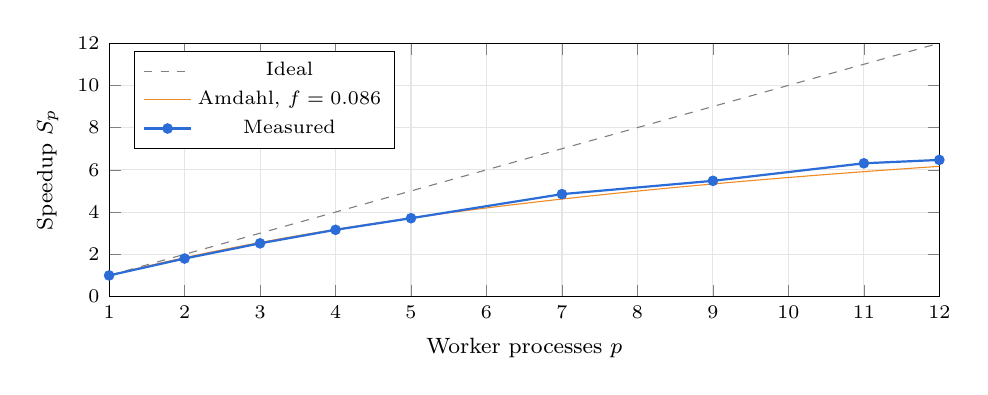
\begin{tikzpicture}
\begin{axis}[
  width=\columnwidth, height=48mm,
  xlabel={Worker processes $p$}, ylabel={Speedup $S_p$},
  xmin=1, xmax=12, ymin=0, ymax=12,
  xtick={1,2,...,12}, ytick={0,2,...,12},
  grid=major, grid style={gray!20},
  legend pos=north west, legend style={font=\scriptsize},
  tick label style={font=\scriptsize}, label style={font=\footnotesize},
]
\addplot[thin, gray, dashed, domain=1:12] {x};
\addlegendentry{Ideal}
\addplot[thin, color=lftrap, domain=1:12, samples=50] {1/(0.086 + (1-0.086)/x)};
\addlegendentry{Amdahl, $f=0.086$}
\addplot[thick, color=lfexit, mark=*, mark size=1.5pt] coordinates
  {(1,1.00)(2,1.80)(3,2.52)(4,3.16)(5,3.71)(7,4.85)(9,5.48)(11,6.31)(12,6.47)};
\addlegendentry{Measured}
\end{axis}
\end{tikzpicture}
\caption{Measured speedup against ideal linear scaling and Amdahl's law with the measured serial
fraction. The demo default is $p=5$.}
\label{fig:speedup}
\end{figure}

\textbf{Task granularity.} At 5 workers, throughput was 1,205 sims/s with chunk size 1, 1,168 with
8, 997 with 180 ($=n/4p$) and 909 with 720 ($=n/p$). Contrary to the common advice to batch small
tasks, the smallest chunks were fastest ($+21\%$ over $n/4p$). A playthrough costs about 3.7\,ms,
much more than dispatching it, but its cost varies between levels and personas, so large chunks
leave some workers idle at the end of a sweep (load imbalance). We therefore changed the default to
small chunks (at most 8). The scaling table above used the earlier $n/4p$ setting, so it is a
conservative estimate.

% =====================================================================
\section{Discussion and Limitations}
% =====================================================================
The agent loop's main benefit over random search is efficiency: equal quality with about a third
fewer simulations, and a modest but consistent gain at equal budget. Its accepted changes are also
interpretable (Table~\ref{tab:case}), which matters when the goal is a fix that a developer
understands. LLM reasoning was comparable to hand-written rules but less consistent; its
advantages are designing levels from scratch, natural-language explanations, and needing no
hand-written playbook, while its costs are API latency and rate limits (425\,s for 4 levels vs.\
seconds offline).

\textbf{Why structured edits?} LLM-written grids can violate hard constraints (uneven rows,
unreachable exits), which is why the generator needs self-correction and deterministic repair. Restricting the LLM to choosing among validated edit operations keeps its
reasoning role (what to change, where, and why) while guaranteeing playability, and makes every
change small enough for a designer to review.

\textbf{Generality.} The framework needs three things from a game: a level representation that
edits can be applied to, a fast simulator with a few player personas, and a complaint taxonomy
mapped to metrics. The agent loop, the parallel engine and the statistics are game-independent, so
the same approach could apply to, for example, platformer or puzzle levels.

\textbf{Threats to validity.} The player agents are rule-based and only approximate human players;
the quality score is a designed proxy and we do not claim it measures fun. The 48 reviews are
synthetic and the problem levels in the main study are procedurally generated stand-ins, so claims
about real players require real reviewed levels. The twin abstracts real-time shooting into
discrete encounters. LLM labelling varies slightly between runs, so each experiment computes the
brief once and shares it across methods. The LLM study used only 4 levels.

% =====================================================================
\section{Conclusion and Future Work}
% =====================================================================
LevelForge takes a level that players complain about, turns their reviews into measurable targets,
and improves the level through an agentic loop backed by parallel simulated play-testing, returning
an optimised level with an explanation the developer can learn from. Critic-guided optimisation
beat random search at equal cost, and multicore simulation made thousands of playthroughs per run
practical on a laptop. Future work: real reviews paired with real levels, a larger LLM study,
learned player models, modelling shooting directly in the twin, multi-objective optimisation (e.g.\
Pareto search) for the trade-offs the LLM struggled with, and a user study with human players.

\bibliographystyle{IEEEtran}
\bibliography{refs}

\end{document}
